\chapter{网络话题的快速生成}\label{chap:topicGeneration}
\section{引言}

随着社交媒体的快速发展,越来越多的用户通过社交媒体来获取信息和分享观点。由此产生了海量的用户生成式数据\citep{pang-2013-unsupervised},使得用户难以从中快速获取热点话题及感兴趣的话题\citep{shahaf2010connecting}。话题是某个种子事件及其相关报道的集合。网络话题检测任务\citep{pang-2013-unsupervised, zhang2013cross}自动地将网络数据组织成更多有意义的热门话题。从本质上来讲,网络话题检测就像从大海里捞针,类比从大量的网络数据中找到一小部分感兴趣数据并将其组织成热门事件\citep{pang-2013-unsupervised}。

传统的话题检测与追踪任务\citep{allan-1998-TDT}致力于将每个新闻报道分配到至少一个话题中\citep{Allan2002Topic}。而这些经过专业编辑的新闻报道数据与网络数据存在极大的差异:由于社交媒体对所发布内容的约束较少,所以来自社交媒体的网络数据更加简短、稀疏并且充满噪声\citep{wxzhao2011comparing};在大量网页中,只有一小部分的网页能够被组织成热点话题\citep{pang-2013-unsupervised}。因此网络话题检测不仅面临着低效的特征表达还需要处理大量的噪声网页。

网络话题检测的关键问题是如何在海量噪声网页存在的前提下组织热点话题。一个直观的方法是在噪声网页存在的情况下去聚类网络话题。然而海量的噪声网页使得传统方法\citep{bojchevski2017RSC,maurus2016skinny,li2007noise}不再适用。为了移除大量噪声网页带来的不利影响,传统的方法\citep{pang-2013-unsupervised,zhang2013cross}采用了一种看似合理的假设:话题内任意一个网页与相同话题内的其他网页之间的相似度应该大于与话题外的网页之间的相似度。然而,这个假设也很难站得住脚,主要问题有以下两个:
\begin{enumerate}
\renewcommand{\labelenumi}{\theenumi)}
    \item 稀疏和充满噪声的网络数据导致低效的特征:用户生成式数据几乎没有受到约束,所以传统的适用于长文本的TF-IDF特征不足以高效表达社交媒体上稀疏的、充满噪声的网络数据。
    \item 低阶特征和高阶语义间存在的语义鸿沟:低阶的特征难以准确地表达高阶语义间的关系。所以网页之间更大的相似度值并不意味着这两个网页在语义上更加相似。
\end{enumerate}

在低效的特征表示以及海量噪声存在的前提下,我们寻找一种无模型且无需复杂参数优化的方法来生成网络话题。首先是因为网络话题的结构和内容差异性很大,一个无模型的方法能拥有好的通用的话题生成能力;其次,为了避免高复杂度的优化措施,一个无需优化的方法能够更好地处理大规模网络数据\citep{pang-tao-2016-lpd};然后,我们避免去处理短文本如何编码生成高效的特征这样一个开放性问题\citep{liu2009topic};最后网络话题检测面临着海量的噪声。

我们研究了网络话题在相似度空间上的统计模式,发现同一个话题下的所有网页之间的相似度与L\'evy Walks存在统计意义上的相似性\citep{perkins2014ascaling}。具体地,我们将网页之间的相似度类比为L\'evy Walks中的步长。那么一个热点话题中的所有相似度的分布大致服从重尾分布,而这重尾分布又是L\'evy Walks中步长的特性。L\'evy Walks\citep{viswanathan2001levy,rhee2011levywalk}是一种随机游走模型,其步长服从重尾概率分布。L\'evy Walks中的$flight$定义为一个质点从一个位置无偏移的移动到另一个位置的步长。直观上讲,L\'evy Walks包含许多短步长的$flight$和一些逃脱短步长控制的额外较长步长的$flight$。因此,L\'evy Walks可以用来很好地描述觅食动物的迁徙模式。

当L\'evy Walks被用来组织网络话题,关键问题变成如下几点:
\begin{enumerate}
\renewcommand{\labelenumi}{\theenumi)}
    \item 如何在未知参数下模拟L\'evy Walks中额外较长的步长即较低的相似度边。
    \item 如何确定话题所需要的步长个数即网页个数。
    \item 在组织话题的时候如何确定所选择的这个步长是否能带来好处。
\end{enumerate}
基于上述三个问题,我们提出以下解决方案:
\begin{enumerate}
\renewcommand{\labelenumi}{\theenumi)}
    \item 提出基于L\'{e}vy Walks的话题生成算法(L\'evy Walks-based Topic Generation,LWTG)。该算法模拟L\'evy Walks的特性,通过采用基于种子话题的网页多分配策略,达到除了将网页分配给最相似的种子话题以模拟L\'evy Walks中普遍较短的步长,同时分配到其他几个稍微较小相似度的种子话题以模拟L\'evy Walks中额外较长的步长的目的,从而优雅地避免了不同L\'evy Walks需要不同参数的麻烦。简单的同时效率也很高。
    \item 根据种子话题的平均相似度,使用层级阈值来截断种子话题的生长,产生一系列过完备话题,从而提高话题的召回率。
    \item 定义一种度量网页跟话题相似度的标准,依据该相似度分配话题,满足一定的聚类准则。至于话题准确率是由PD算法\citep{pang-2013-unsupervised,pang-tao-2016-lpd,pang-tao-2018-neurocomputing}通过对话题的兴趣度进行排序来保证的。PD算法在经验上认为话题的精确数量不重要,一小部分热点话题总能被正确排在前面。因此网络话题检测的准确率由PD算法保证。
\end{enumerate}

据我们所知,本论文是第一个发现网络话题检测在相似度空间上和L\'evy Walks具有相似的特点,并且进行了一系列实验来阐述这个发现所带来的好处。我们提出的LWTG算法不仅简单快速,而且能够进一步提高话题的召回率。通过简单地对网页进行分配,无需复杂的参数优化,我们找到了一种新的组织网络话题的方法。我们的方法在网络话题的生成效率方面已经远超当前最好的方法,而且在网络话题召回率方面也能够赶上甚至超越当前最好的方法。算法框架如图\ref{fig:topic_generation_process}所示。
\begin{figure}[!htbp]
    \centering
    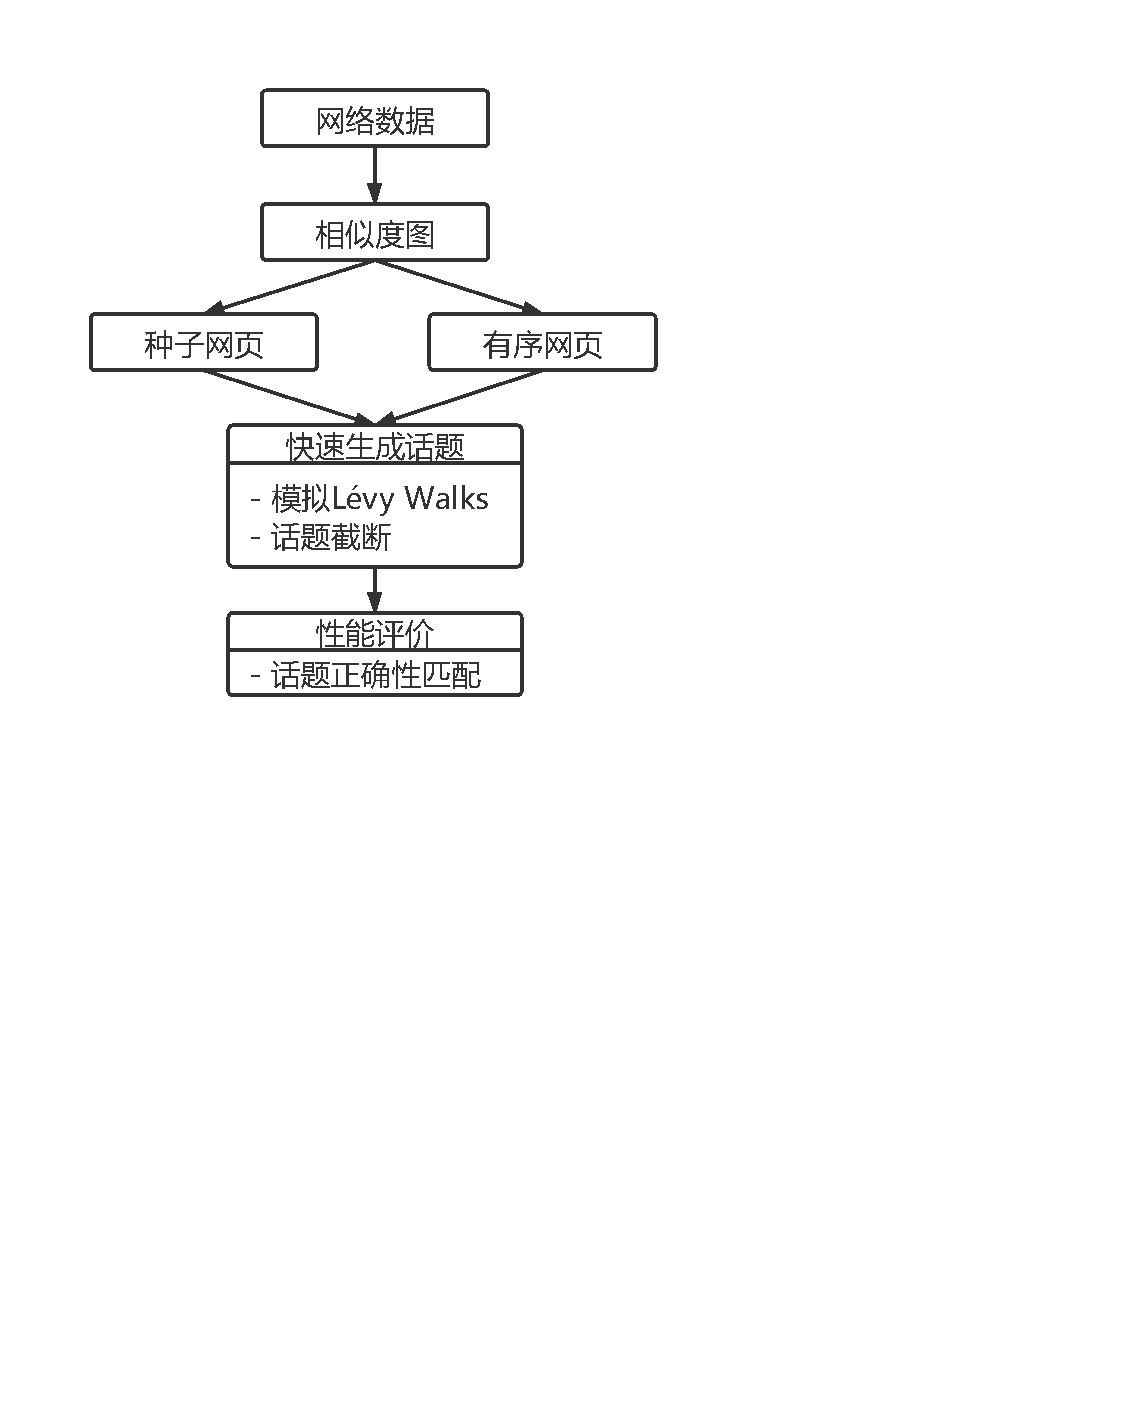
\includegraphics[width=0.70\textwidth]{topic_generation_process}
    \caption{通过模拟L\'evy Walks来快速生成网络话题的流程图}
    \label{fig:topic_generation_process}
\end{figure}

\section{相似度图的构建}\label{sec:constructsimilaritygraph}

本章的研究重点是网络话题的快速生成。因此,为了减少其他因素的影响,我们忽略网络数据的多模态性和时间戳、链接等其他信息,只使用纯文本信息。所以每个网页就是一个文本字符串。对于给定的网络数据集,包含一系列的网页$W=\{w_1,...,w_N\}$,我们对其进行处理,生成一个$k$近邻($k$-Nearest Neighbor,$k$-N$^2$)的相似度图$G=(V,E,A)$。其中顶点集$V$对应网页集合$W$,仿射矩阵$A$($a_{ij}\in A$)对应截断后任意两个网页之间的相似度,边集$E$($e_{ij}\in E$)对应任意两个网页之间的非$0$边\citep{pang-2013-unsupervised,pang-tao-2016-lpd}。具体处理如下。

首先,我们对网页的文本字符串进行分词。然后使用词袋模型\citep{harris1954distributional}对网页文本进行基本的统计和表示,再用TF-IDF特征值表示每个词的权重,这样每个网页就可以用一个特征向量$x_i\in \mathbb{R}^M(i=1,...,N)$表示。其中M是表示词典大小,N表示网络数据集中网页的数量。对于TF-IDF特征,TF表示词频,IDF表示逆文档频率。一个词在文档中出现的频率越高,其词频值越大,相应TF-IDF值就越大。与此同时,一个词如果出现在越多的文档中,则其逆文档频率值越低,相应TF-IDF特征值就越低。逆文档频率降低那些高频出现但是较没有判别意义的词的权重。比如:‘我’、‘那’这种指示代词几乎没有判别能力,虽然它们的词频值很大,但是它们的逆文档频率值很低,进而使得TF-IDF值很低。虽然还可以使用更高级的特征,但是语义鸿沟问题仍然存在,而且使用TF-IDF特征足够简单,能够带来更快的处理速度。

然后,基于得到的每个网页的特征向量,我们可以通过余弦距离来度量两个网页之间的相似度大小。在公式\ref{eq:cosinedistance}中,$S_{ij}$表示两个网页之间的初始相似度,$x_i$和$x_j$表示两个网页的特征向量:
\begin{equation}\label{eq:cosinedistance}
    S_{ij} = \frac{x_i\cdot x_j}{|x_i||x_j|}
\end{equation}

最后,得到相似度图后,在每个网页中,保留与其语义最相近的$k$个网页关系,删除其他网页关系。这里假设两个网页之间相似度越高则语义越相近。这样做能够过滤掉大量网页之间的噪声干扰,即不相关的噪声网页。网络数据集中的噪声网页越多,$k$应该选择更低的值。在公式\ref{eq:knn}中$KNN(w_i)$表示与网页$w_i$语义最相近的$k$个网页集合。同时,我们使用公式\ref{eq:filtergraph}将两个网页之间低于某个阈值$\epsilon$的相似度置为$0$,因为我们认为过低的相似度表示这两个网页在语义上已经没有关联关系了。这进一步过滤了噪声网页。
\begin{equation}\label{eq:knn}
S_{ij} =
\begin{cases}
0, &  w_j \notin KNN(w_i) \\
S_{ij}, & w_j \in KNN(w_i)
\end{cases}
\end{equation}

\begin{equation}\label{eq:filtergraph}
a_{ij} =
\begin{cases}
0, & S_{ij} < \epsilon \\
S_{ij}, & S_{ij} \geq \epsilon
\end{cases}
\end{equation}


\section{网络话题的L\'{e}vy Walks特性}

\begin{definition}
    网络话题的相似度空间

    给定一个由网页数据集构建的$k$-N$^2$图$G=(V,E,A)$和一个话题$C$,网络话题$C$的相似度空间定义为
    一系列相关联的边$e_{ij}$经过仿射后的相似度$a_{ij}$,其中网页$w_i$和$w_j$至少有一个属于该话题。
\end{definition}

网络话题的相似度空间包含两种相似度:1)话题内部相似度:同个话题内部两个网页之间的相似度;2)话题之间相似度:两个不在同个话题内的网页之间的相似度。

\begin{figure}[!htbp]
    \centering
    \begin{subfigure}[b]{0.5\textwidth}
      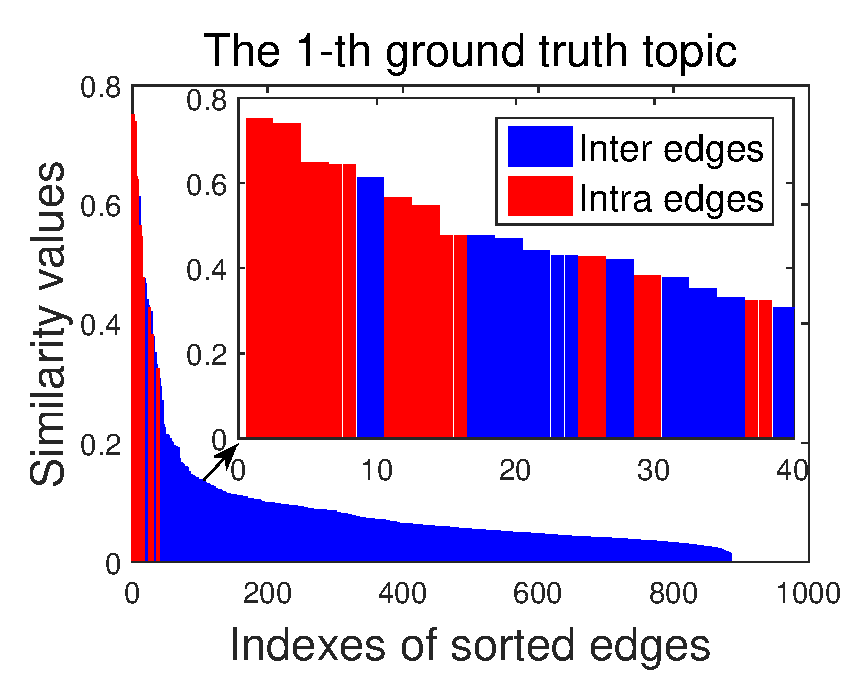
\includegraphics[width=\textwidth,height=0.9\textwidth]{barGraph_topic_1}
      \caption{}
      \label{fig:barGraph_t1}
    \end{subfigure}%
    % ~% add desired spacing
    \begin{subfigure}[b]{0.5\textwidth}
      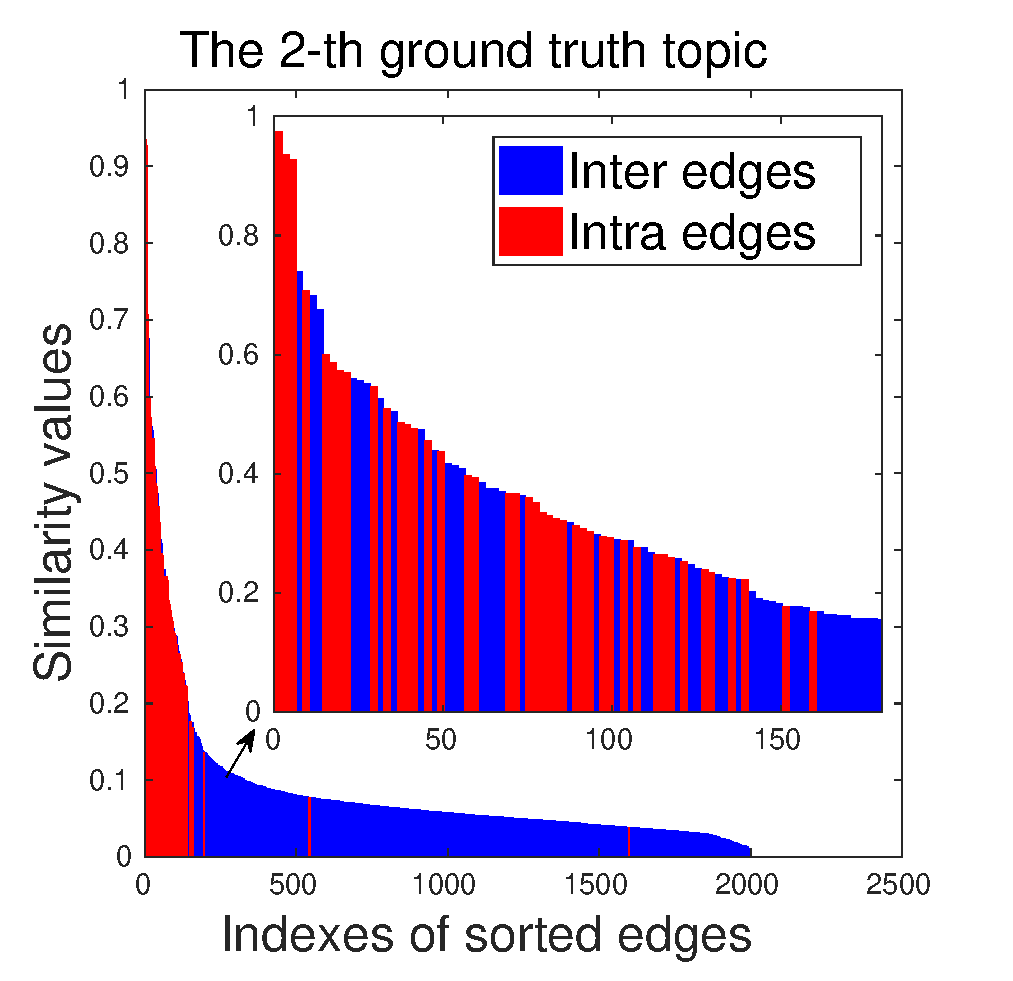
\includegraphics[width=\textwidth,height=0.9\textwidth]{barGraph_topic_2}
      \caption{}
      \label{fig:barGraph_t2}
    \end{subfigure}
    % \\% line break
    \begin{subfigure}[b]{0.5\textwidth}
      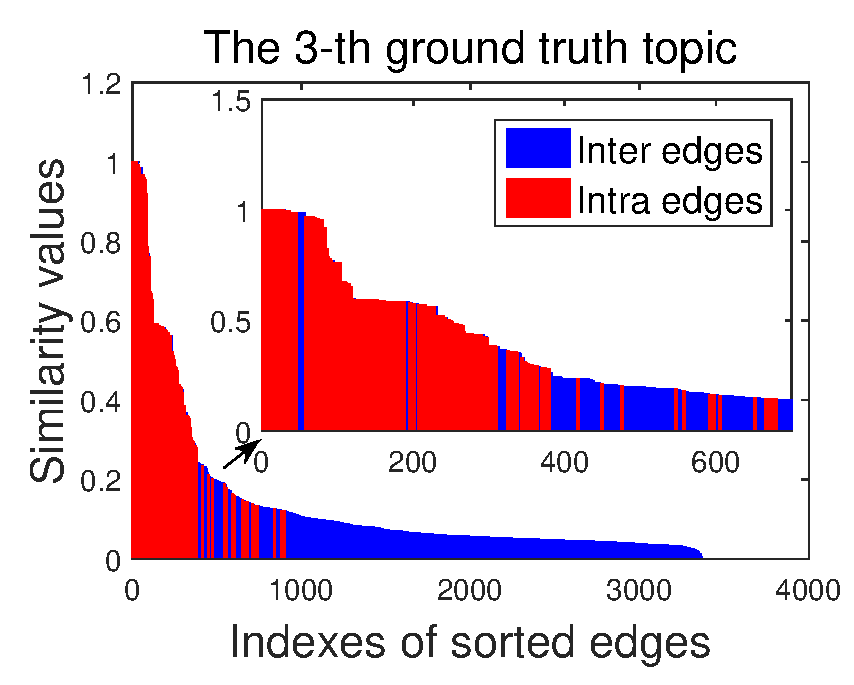
\includegraphics[width=\textwidth,height=0.9\textwidth]{barGraph_topic_3}
      \caption{}
      \label{fig:barGraph_t3}
    \end{subfigure}%
    % ~% add desired spacing
    \begin{subfigure}[b]{0.5\textwidth}
      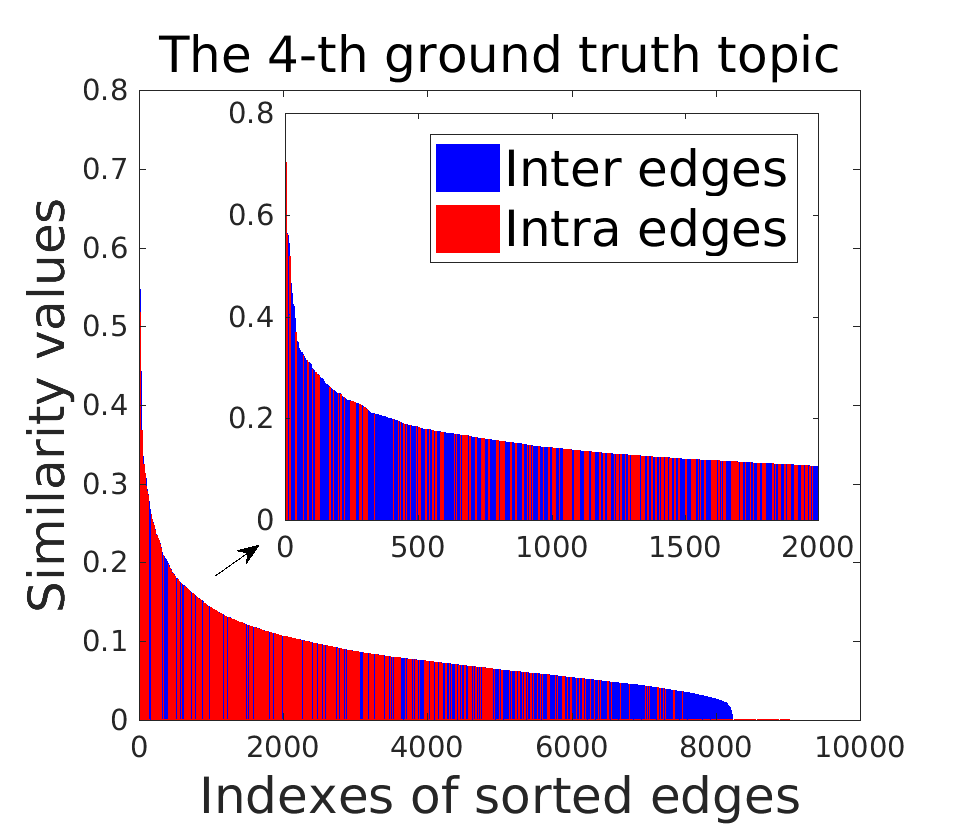
\includegraphics[width=\textwidth,height=0.9\textwidth]{barGraph_topic_4}
      \caption{}
      \label{fig:barGraph_t4}
    \end{subfigure}
    \caption{四个真实网络话题的相似度空间}
    \label{fig:barGraph}
\end{figure}
我们从MCG-WEBV数据集中随机选择四个真实的网络话题来理解网络话题在相似度空间上的模式。对同个话题内部的相似度进行从大到小排序。图\ref{fig:barGraph}展示了这四个网络话题的相似度空间。

\begin{figure}[!htbp]
    \centering
    \begin{subfigure}[b]{0.5\textwidth}
      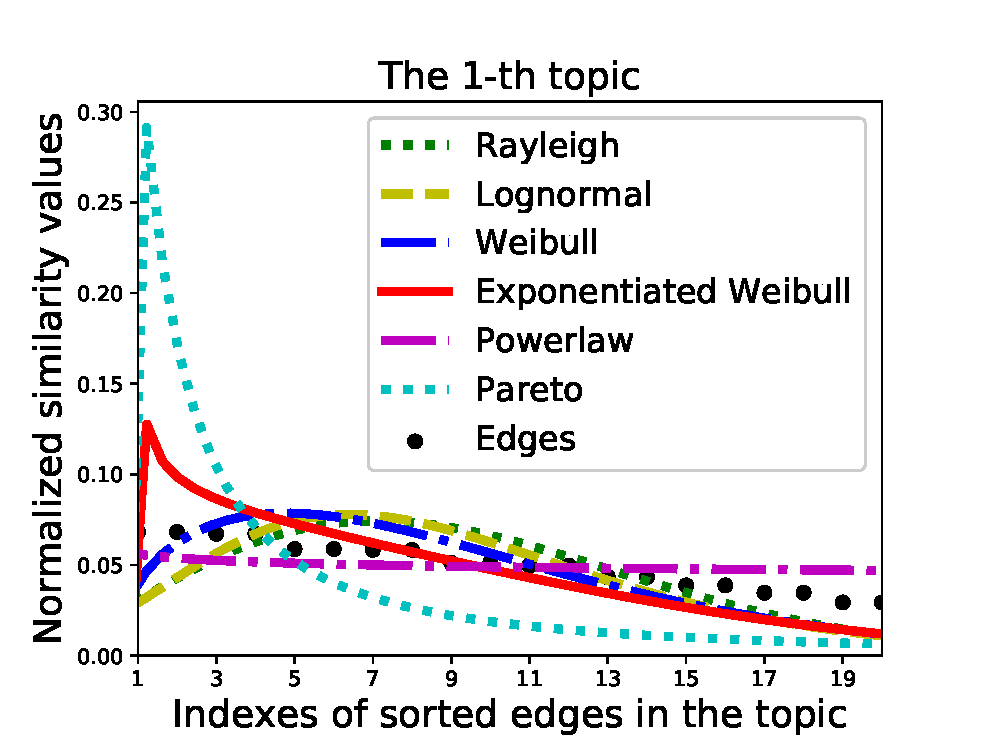
\includegraphics[width=\textwidth,height=0.8\textwidth]{fit_distribution_topic_1}
      \caption{与指数韦伯分布函数拟合最好}
      \label{fig:fitdistribution_t1}
    \end{subfigure}%
    % ~% add desired spacing
    \begin{subfigure}[b]{0.5\textwidth}
      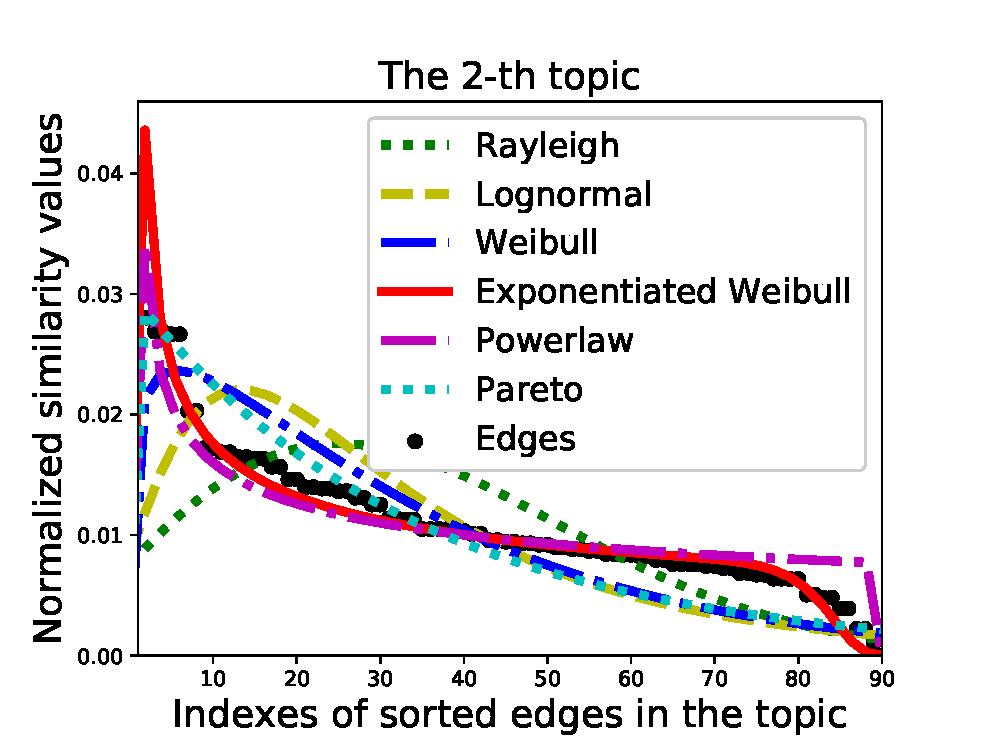
\includegraphics[width=\textwidth,height=0.8\textwidth]{fit_distribution_topic_2}
      \caption{与幂次分布函数拟合最好}
      \label{fig:fitdistribution_t2}
    \end{subfigure}
    % \\% line break
    \begin{subfigure}[b]{0.5\textwidth}
      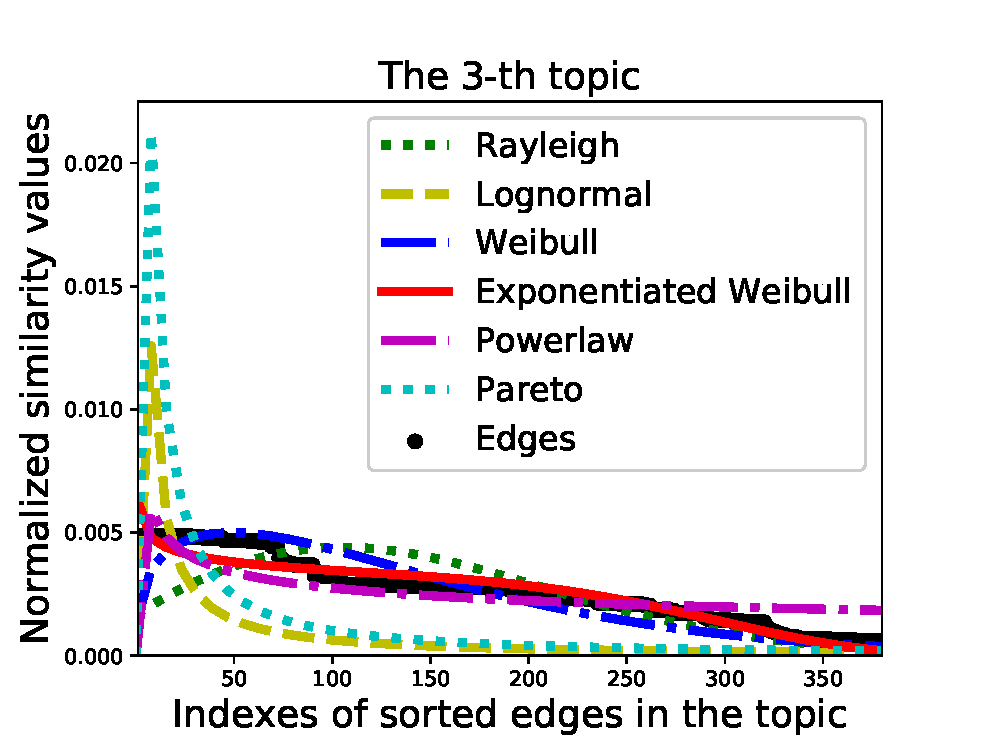
\includegraphics[width=\textwidth,height=0.8\textwidth]{fit_distribution_topic_3}
      \caption{与指数韦伯分布函数拟合最好}
      \label{fig:fitdistribution_t3}
    \end{subfigure}%
    % ~% add desired spacing
    \begin{subfigure}[b]{0.5\textwidth}
      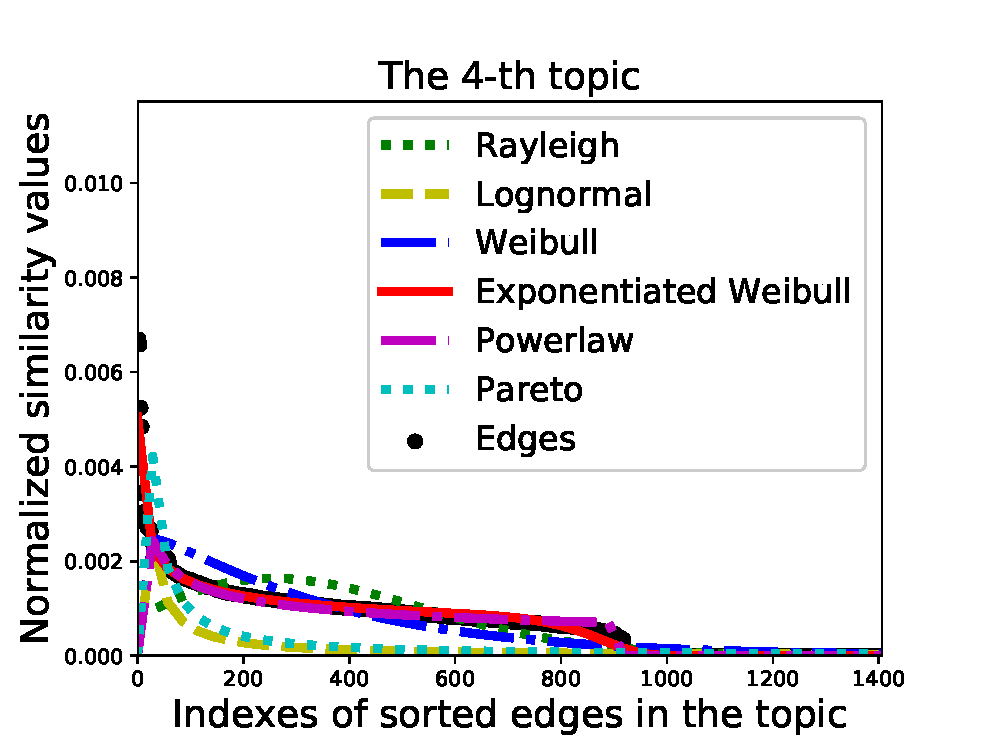
\includegraphics[width=\textwidth,height=0.8\textwidth]{fit_distribution_topic_4}
      \caption{与幂次分布函数拟合最好}
      \label{fig:fitdistribution_t4}
    \end{subfigure}
    \caption{四个真实网络话题在相似度空间中拟合重尾分布函数}
    \label{fig:fitdistribution}
\end{figure}
同时,对于这四个网络话题,我们将每个话题内的所有相似度归一化排序后进行分布函数拟合,从图\ref{fig:fitdistribution}可以看出话题内已排序的相似度服从重尾分布。此时,有两个问题需要确定:
\begin{enumerate}
\renewcommand{\labelenumi}{\theenumi)}
    \item 是否所有的话题服从相同的重尾分布?
    \item 服从相同分布的话题是否拥有相同的分布参数?
\end{enumerate}

为了解决上述问题,我们使用极大似然估计去将已排序的相似度拟合为已知的分布。例如:指数韦伯分布、锐利分布、韦伯分布、对数正态分布、幂次分布、帕累托分布。表\ref{tab:PDF}列出这些分布的概率密度函数。而且,为了量化最好的分布,我们引入赤池信息准则(Akaike\'s Information Criterion,AIC)\citep{burnham2004multimodel}:
\begin{equation}\label{eq:AIC}
 \text{AIC} = -2log(L(\hat{\theta}|data)) + 2K
\end{equation}
其中$L(\cdot)$是似然函数,K是参数的数量。由于AIC值容易受样本大小影响\citep{rhee2011levywalk},不能被直接用来作为绝对的度量标准。所以,使用下面的转换形式作为每个模型的置信权重\citep{burnham2004multimodel}:
\begin{equation}\label{eq:AICweight}
    w_i = \frac{exp(-\Delta_i/2)}{\sum_{r=1}^{R}exp(-\Delta_r/2)}
\end{equation}
其中R是分布函数数量。$\Delta_i=\text{AIC}_i-\text{AIC}_{min}$,$\text{AIC}_{min}$是不同AIC值中的最小值。赤池信息权重被认为是分布函数可能性的归一化值。
\begin{table}[!htbp]
    \caption{常见的重尾分布函数。}
    \label{tab:PDF}
    \centering
    % \footnotesize% fontsize
    \setlength{\tabcolsep}{4pt}% column separation
    \renewcommand{\arraystretch}{1.2}%row space
    \begin{tabular}{|c|c|}
        \hline
        分布函数 & 概率密度函数\\
        \hline\hline
        指数韦伯分布$^1$ & $(1-\exp(-\frac{x}{\lambda})^k)^{\alpha}$\\
        \hline
        锐利分布 & $\frac{x}{\sigma^2}\exp(\frac{-x^2}{2\sigma^2})$\\
        \hline
        韦伯分布$^2$ & $\frac{k}{\lambda}(\frac{x}{\lambda})^{k-1}\exp(-(\frac{x}{\lambda})^k)$\\
        \hline
        对数正态分布 & $\frac{1}{x\sigma\sqrt{2\pi}}\exp(-\frac{\ln(x)-\mu}{2\sigma^2})$\\
        \hline
        幂次分布 & $a(cx)^{-k}$\\
        \hline
        帕累托分布$^3$ & $\frac{\alpha a^{\alpha}}{x^{\alpha+1}}$\\
        \hline
    \end{tabular}\\
    \footnotesize{$^1$ $\alpha \geq 1.$}\\
    \footnotesize{$^2$ $k < 1.$}\\
    \footnotesize{$^3$ $0 < a \leq x$}\\
\end{table}

从图\ref{fig:barGraph}到\ref{fig:fitdistribution},我们可以得到下面观察结果:
\begin{enumerate}
    \item[1)] 相同话题下网页之间的已排序的相似度与L\'evy Walks存在统计意义上的相似特性。图\ref{fig:fitdistribution}表明同个话题内的相似度服从重尾分布。
    \item[2)] 不同的话题服从不同的重尾分布。例如,根据赤池信息置信权重公式\ref{eq:AICweight},图\ref{fig:fitdistribution_t1}所表示的第一个话题服从指数韦伯分布,而图\ref{fig:fitdistribution_t2}所表示的第二个话题服从幂次分布。
    \item[3)] 热点话题中包含一些额外的边。如图\ref{fig:barGraph}所示,如果话题的相似度按照递减排序,那么由边连接排在较前的网页,并不意味其绝对属于该话题。
\end{enumerate}

如果将相似度类比为网页之间的步长,那么与L\'evy Walks相比,网络话题在相似度空间上有两个统计意义上的相似特性:1)L\'evy Walks中的步长和网络话题的相似度均服从重尾分布;2)L\'{e}vy Walks和网络话题均包含许多较短的步长(较高相似度)和一些额外较长的步长(较低相似度)。至此,这两个相似特性被认为是网络话题的L\'evy Walks特性。

\section{通过模拟L\'evy Walks生成话题}

既然网络话题有L\'evy Walks特性,我们试图从这个特性入手,从海量网络数据中生成话题。一个最简单的办法是根据重尾分布来组织网页进入对应话题。然而,正如之前所言,我们不可能提前训练一个通用的含有重尾分布函数的模型。

通过在相似度空间利用重尾分布的特点,我们认为可以在将网页分配给话题的时候适当添加一定的随机性以模拟L\'evy Walks中额外较长的步长(较低的相似度)。为此,我们设计了一种通过模拟L\'evy Walks来生成话题的算法(L\'evy Walks-based Topic Generation,LWTG)。LWTG算法的框架如图\ref{fig:LWTG}所示。
\begin{figure}[!htbp]
    \centering
    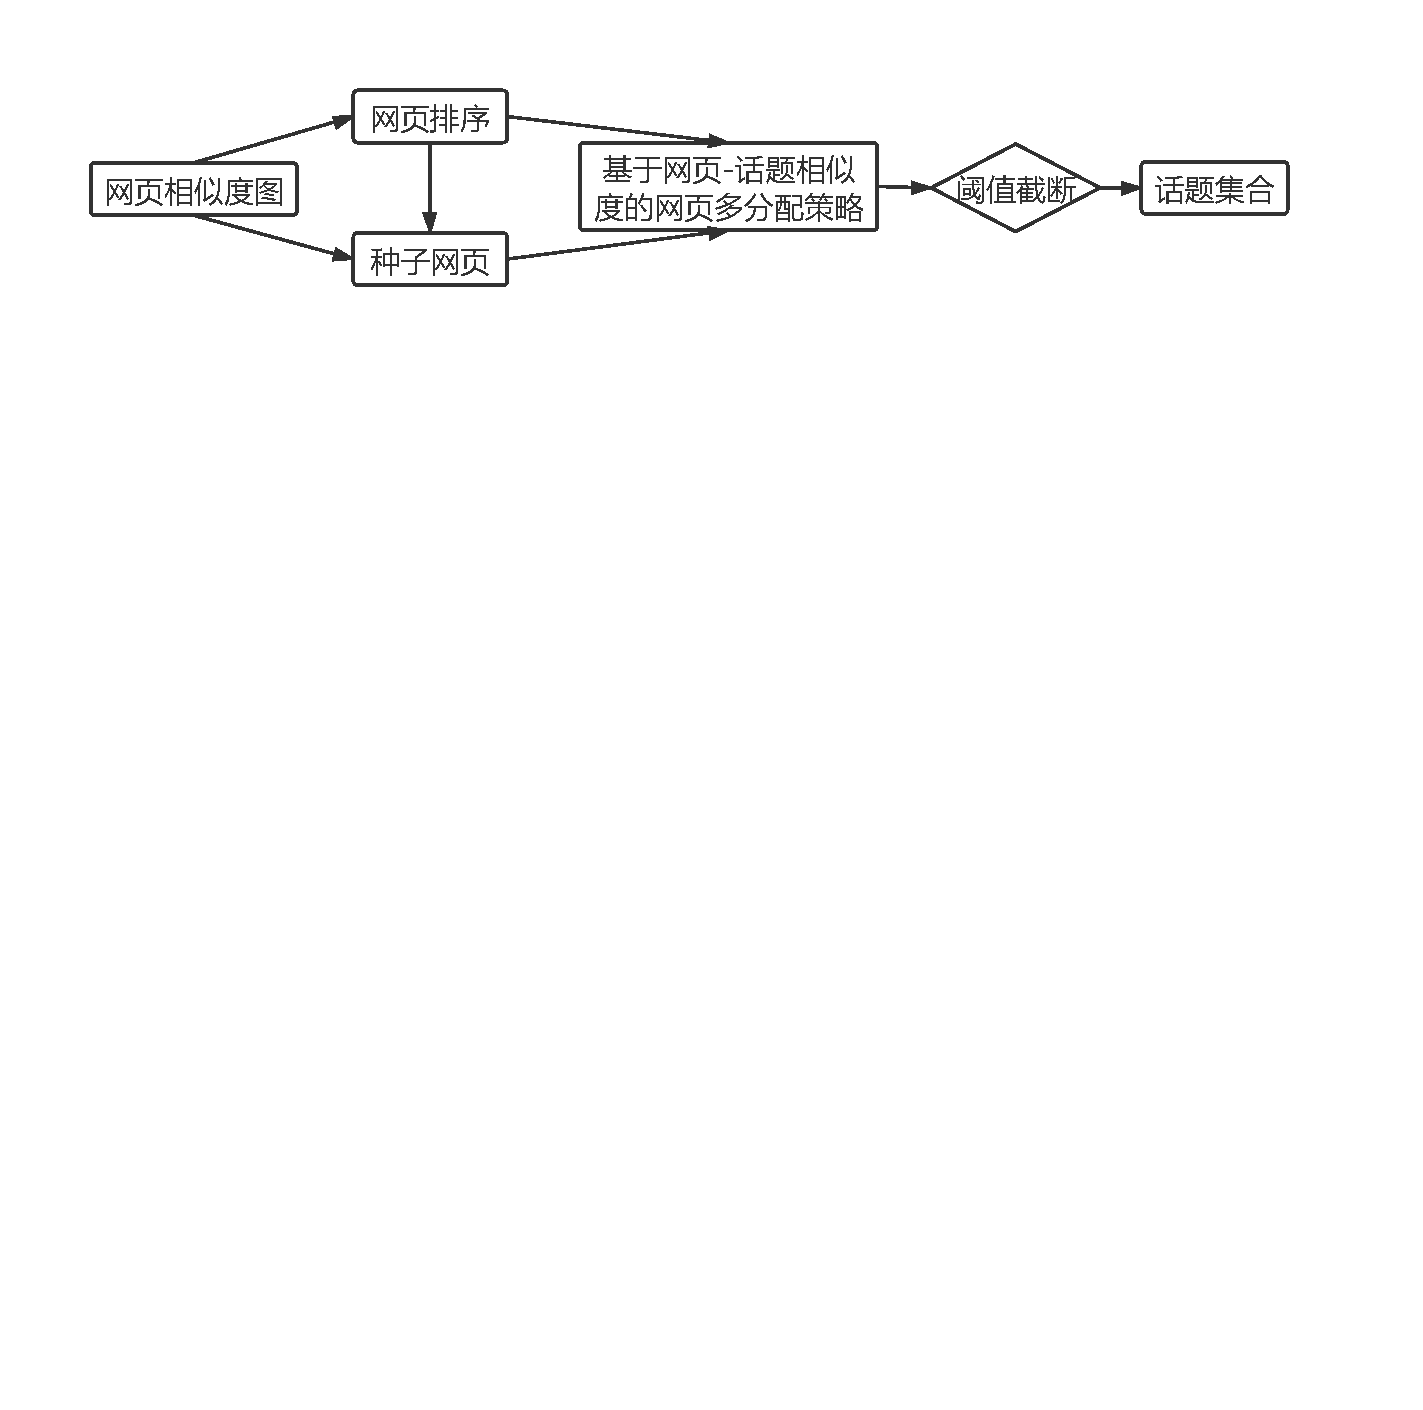
\includegraphics[width=1.0\textwidth]{LWTG}
    \caption{LWTG算法生成网络话题的框架图}
    \label{fig:LWTG}
\end{figure}

本论文中,我们定义一种度量网页和话题相似度的方法,并将网页分配给相似度最高的$K$个话题。这样,除了相似度最高的话题满足聚类准则外,其他$K-1$话题用来模拟网络话题在相似度空间中的L\'evy Walks特性:一些额外较低的相似度。

\subsection{寻找种子网页}
\begin{figure}[!htbp]
    \centering
    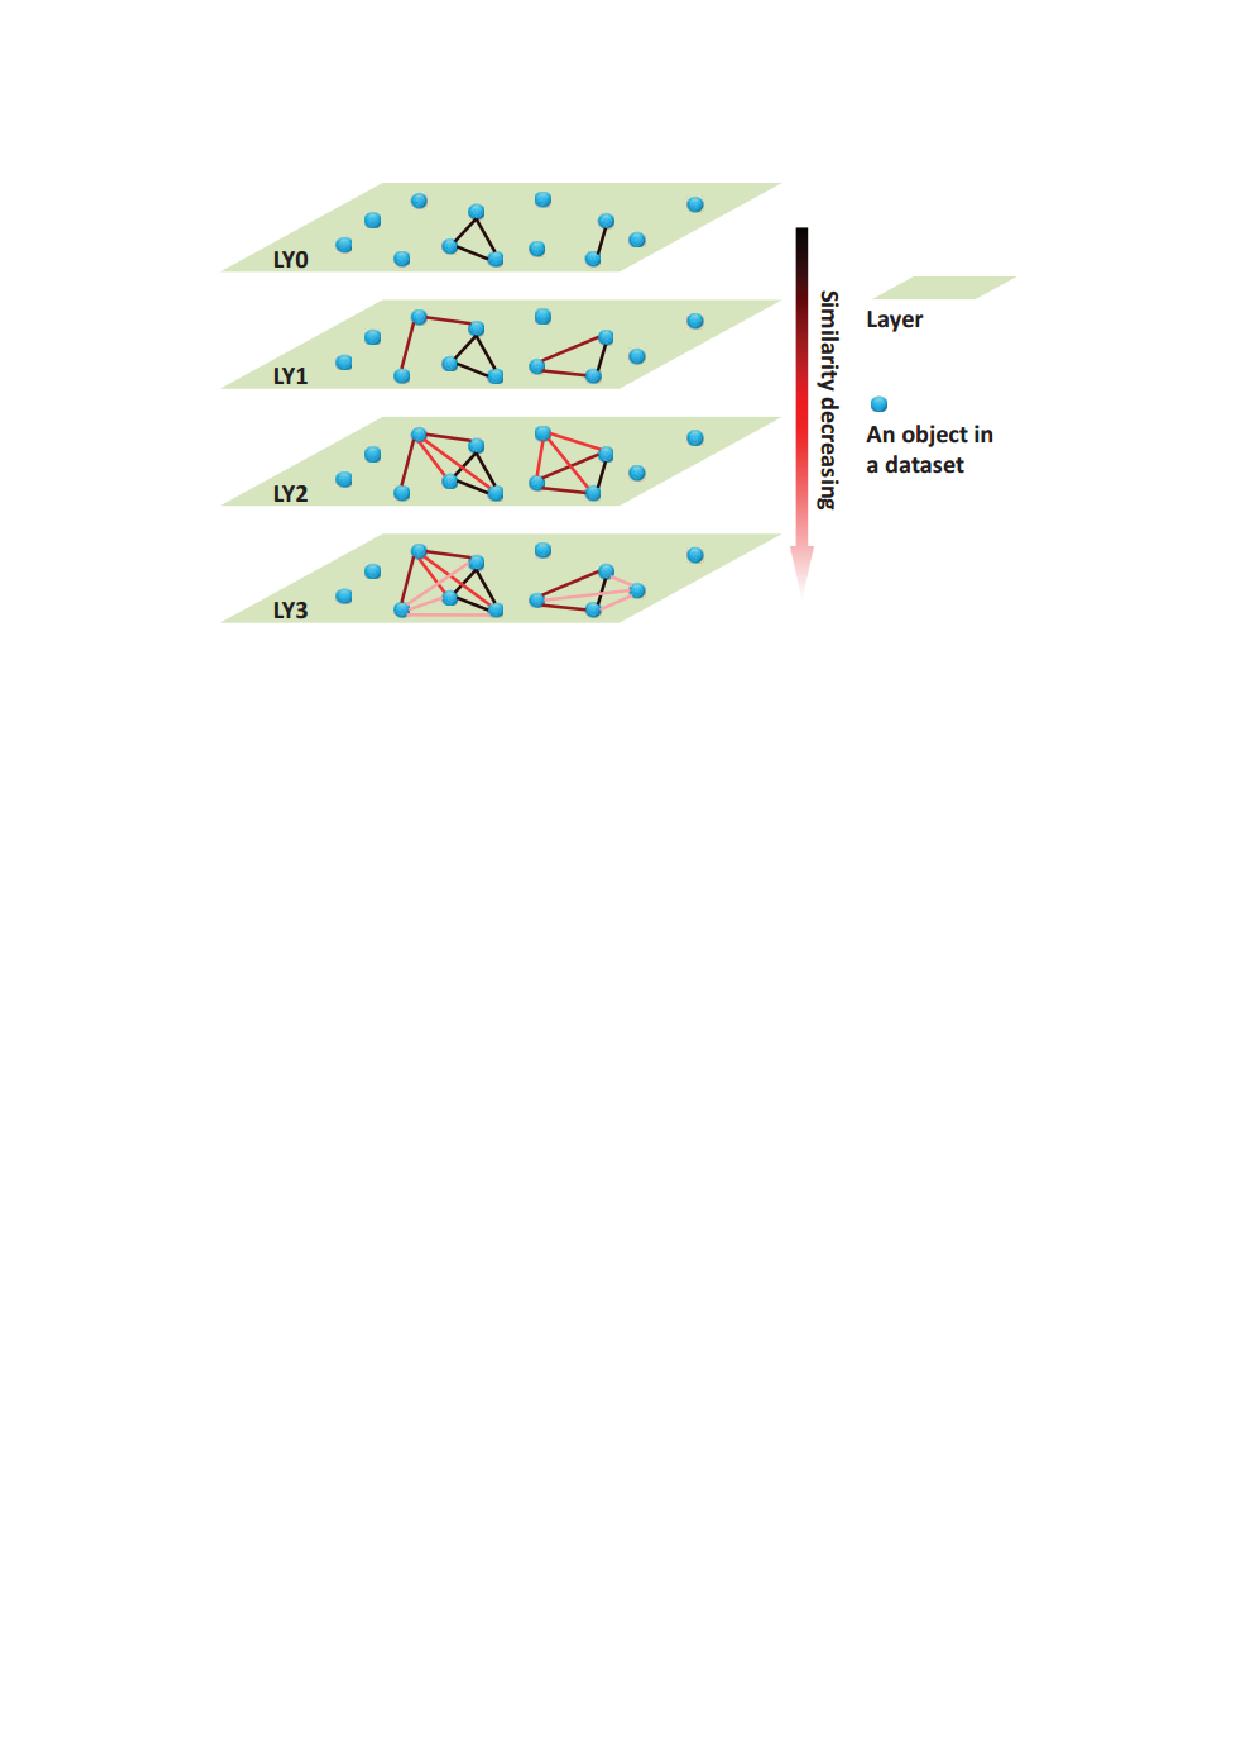
\includegraphics[width=1.0\textwidth]{similarity_cascade.pdf}
    \caption{基于相似度流的网络话题演化示意图}
    \label{fig:similarity_cascade}
\end{figure}
网络话题由初始核心事件不断在社交媒体上传播得以发展壮大。传播过程会逐渐吸收许多直接或者间接的外延信息。
网络话题的形成可以被看做是一种信息扩散的过程。而信息扩散的过程肯定会有一定的损失。我们使用相似度流来模拟这种信息扩散过程,扩散过程中信息的损失对应于相似度流中相似度值的减小。图\ref{fig:similarity_cascade}展示了网络话题基于相似度流的演化过程:话题初始时只有一两个网页,随后在较低的相似度上吸收更多的网页来形成更大的话题。随着演化的进行,吸收的网页的相似度越来越低。这种过程我们称之为相似度流扩散(Similarity Cascade, SC)。又因为不同用户之间的需求是不一样的,导致用户对话题的理解具有极大的差异。所以对同一个核心事件演化形成的话题,不同的用户所理解的话题的规模也是不一样的。

既然话题是由核心事件演化来的,那么我们希望能够通过代表该核心事件的种子网页,进而通过相似度流的扩散过程来模拟演化过程,最终生成话题。首要问题是如何判断一个网页能否作为种子网页?直观上理解,在一个由多个网页构成的话题中,其网页分布应该是尽可能均匀且紧凑的\citep{liu2014entropy}。均匀表示该话题内的网页之间的相似度较为接近,这是因为话题内的网页都是在为该话题服务的,所以它们应该是相似的,即相似度应该尽可能一致。紧凑表示该话题内的网页与话题应该是紧密相关,即相似度应该尽可能大。

受到论文\citep{wang2010measuring}的启发,我们引进了站点熵率(Site Entropy Rate,SER)用来度量网页成为种子网页的概率。通过将相似度流从一个网页转移到另一个网页的过程模拟为全连接图中从一个站点转移到另一个站点的随机游走的过程,SER意味着从一个网页在一步内转移到其他网页的平均总信息转移量。而由种子网页吸收相似网页演化生成话题的过程中,越接近初始核心事件的网页,其通过相似度能够转移的平均总信息量也越大。SER的公式如下:
\begin{equation} \label{eq:SER}
\text{SER}_i = \pi_i\sum_{j\in<i>}-P_{ij}\log P_{ij}
\end{equation}
其中$P_{ij}=\frac{a_{ij}}{\sum_{j\in <i>}a_{ij}}$表示网页$w_i$转移到网页$w_j$的转移概率。$<i>\subset[1:N]$保存了s个与网页$w_i$最相似的网页索引。
公式\ref{eq:SER}表明SER可以被分为两个部分:稳态分布项和熵项。这两部分作用分别如下:
\begin{enumerate}
  \item[1)] 稳态分布项:$\pi_i = \frac{a_i}{a}$,其中$a_i=\sum_{j\in<i>}a_{ij}$是从网页$w_i$出发到s个最相关网页的相似度的和,$a = \sum_{i}\sum_{j\in<i>}a_{ij}$是相似度图中的所有网页及其最相似的s个网页的相似度的和。$\pi_i$被认为是网页$w_i$访问其他网页的频率,$\pi_i$越大,则表示由网页$w_i$经过一步演化的话题更加的紧凑;
  \item[2)] 熵项:$\sum_{j\in<i>}-P_{ij}\log P_{ij}$度量了网页$w_i$在一步内访问其他网页的不确定性。熵项越大,表明与网页$w_i$直接相连的其他网页的相似度分布更加均匀。
\end{enumerate}

\begin{figure}[!htbp]
    \centering
    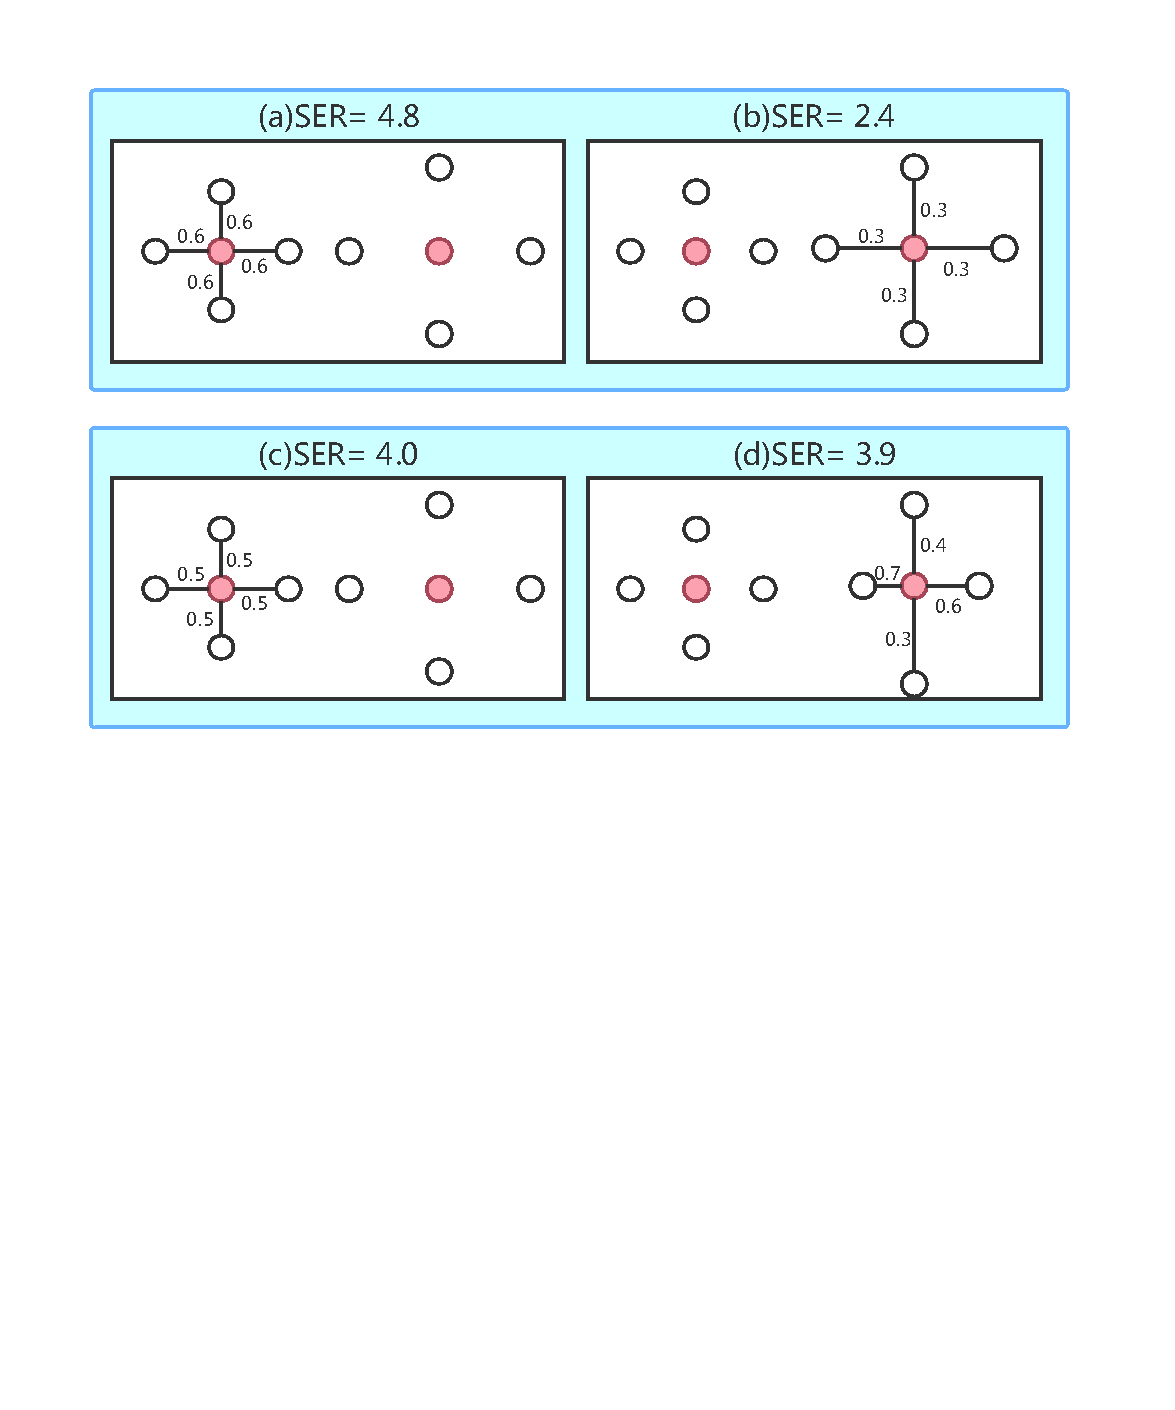
\includegraphics[width=1.0\textwidth]{seed_web_entropy.pdf}
    \caption{网页一步演化成话题的紧凑性和均匀性的SER评估}
    \label{fig:seed_web_entropy}
\end{figure}
SER由这两项的乘积构成。网页的SER越大,则表示其越有可能成为话题中的中心网页。如图\ref{fig:seed_web_entropy}所示,图中空心圈圈表示网页,红色实心圆圈表示要评估的网页,数字表示网页之间的相似度。从图(a)和图(b)可以看出在相同均匀分布的情况下(熵项一致),相似度分布越紧凑的网页有更大的SER值。从图(c)和图(d)可以看出在相同紧凑性情况下(稳态分布项$\pi$一致),相似度分布越均匀的网页有更大的SER值。

定义了SER作为网页成为种子网页的概率后,我们提出了一种基于关联度的种子网页贪心搜索算法来找到不同规模的种子网页。算法\ref{alg:greedysearchseedweb}展示整个种子网页的搜索过程。算法的输入为$k$近邻相似度图。然后根据相似度图来计算每个网页的SER值。这里我们只需要选择与网页最相似的$s$个网页的相似度来计算SER值即可。因为SER仅用作一步内的相似度转移,而在一步内转移的网页应该是比较相似且数量比较少的,而不是全部的网页。所以这里我们只选择了$s$个最相似的网页来计算SER的值。另一个关联度参数$d$在搜索过程中用来确定与当前网页最相似的$d$个网页。只有在当前网页及其最相似的$d$个网页均未被标记的情况下,当前网页才被选作种子网页,同时过滤当前网页及其最相似的$d$个网页。这么做是因为我们认为这d个最相似的网页与当前网页同属于一个话题,是话题内部最紧密的关系,可以相互演化扩展。d值越大,就会过滤掉越多的相关网页,最终产生的种子网页数量就会越少。由于d值不好确定,同时为了更好地提高话题的召回率,我们使用多个不同的d值来产生多种规模的种子网页。算法输出为规模较小的种子网页集合。整个算法是基于SER值排序的贪心过滤算法:按SER值从大到小的顺序逐一判断每个网页,如果当前网页及其最相似的d个网页均未被过滤,则确定当前网页为种子网页,并且过滤当前网页及其最相似的d个网页。
\begin{algorithm}[!htbp]
    % \small
    \caption{基于关联度的种子网页贪心搜索算法}\label{alg:greedysearchseedweb}
    \hspace*{0.02in}{\bf Input:}
    相似度图 $G=(V,E,A)$,最相似网页个数$s$,关联度$d$\\
    \hspace*{0.02in}{\bf Output:}
    种子网页集合 $SW$,有序网页索引$SortedIndex$
    \begin{algorithmic}[1]
        % \State 初始化网页访问与否的的标记向量visit$\in \mathbb{R}^{N}$为False
        \State 初始化最终要生成的种子网页集合$SW$为空集
        \State 根据公式\ref{eq:SER}计算所有网页的SER
        \State 根据SER进行从大到小排序,得到有序且有连接的网页索引$SortedIndex$
        \For{$i \in SortedIndex$}
        \State 找出与每个网页$w_i$最相似的$d$个网页索引,记为$\{i\}$
        \If{网页$w_i$ 及其最相似的$d$个网页$w_{\{i\}}$ 均未被过滤}
        \State $SW \leftarrow SW \bigcup w_i$
        \State 标记网页$w_i$及其最相似的$d$个网页$w_{\{i\}}被过滤$
        \EndIf
        \EndFor
    \end{algorithmic}
\end{algorithm}


\subsection{网页多分配算法}

\begin{algorithm}[!htbp]
    % \small
    \caption{基于种子话题的网页多分配算法}\label{alg:multiallocateweb}
    \hspace*{0.02in}{\bf Input:}
    相似度图$G=(V,E,A)$,网页索引$SortedIndex$,种子网页集合$SW$,$K$\\
    \hspace*{0.02in}{\bf Output:}
    一系列话题集合$C$
    \begin{algorithmic}[1]
        \State 初始化空的话题集合C
        \State 初始化种子话题$C_s$($s\in SW$)及对应的阈值$th_s=1$
        \For{$i \in SortedIndex$}
        \State 根据公式\eqref{eq:avgrate}计算$S_{is}$\Comment{计算网页$w_i$与所有种子话题的相似度}
        \State $\{i\} \leftarrow \operatorname*{argmaxk}\limits_{s\in SW}(S_{is}, K)$\Comment{取与网页$w_i$最相似的$K$个种子话题的索引}
        \For{$s \in \{i\}$}
        \If{$IsCut(C_s, w_i, th_s)}$
        \State $C \leftarrow C \bigcup C_s$\Comment{截断种子话题生长,生成一个话题}
        \State $C_s \leftarrow C_s \bigcup w_i$\Comment{更新种子话题}
        \State $th_s = \lfloor{\text{Avg}(C_s)\times10}\rfloor\div 10$\Comment{更新层级阈值}
        \EndIf
        \EndFor
        \EndFor
    \end{algorithmic}
\end{algorithm}

在产生种子网页后,我们提出了网页多分配算法来实现种子网页吸收相似网页,进而演化成话题。我们通过将网页分配给相似度最高的$K$个话题来模拟网络话题L\'evy Walks特性中额外较低的相似度。同时这个分配过程模拟了相似度流的扩散过程,所以我们采用了生成种子网页过程中产生的网页遍历顺序作为我们遍历网页的顺序。对于非噪声的有边连接的网页,逐个进行分配。算法\ref{alg:multiallocateweb}展示了这个分配过程。其中对于每个待分配的网页,我们需要计算其与种子话题的相似度,希望这个相似度能够反映种子话题对网页的吸引程度。我们定义网页$w_i$对种子话题$C_s$的相似度为该网页所带来的平均相似度对比种子话题$C_s$当前平均相似度的比例。如公式\ref{eq:avgrate}所示,Avg($\cdot$)为取平均函数。我们认为网页$w_i$如果能给种子话题$C_s$带来所增加的相似度的平均值的比例越高,那么网页$w_i$与种子话题$C_s$必然更加密切相关。即网页$w_i$就有更大的可能性归属于该种子话题$C_s$。
\begin{equation}\label{eq:avgrate}
  S_{is} = \frac{\text{Avg}\big(\sum_{j\in C_s}(a_{ij}+a_{ji})\big)}{\text{Avg}(C_s)}
\end{equation}

得到网页与种子话题的相似度后,我们将网页分配给相似度最高的$K$个种子话题。公式\ref{eq:iscut}实现了函数$IsCut(\cdot)$,其中$th_s$使用了层级阈值来截断种子话题,从而生成过完备的话题。阈值$th_s$在每一轮更新种子话题后重新赋值为当前种子话题的平均相似度所处的那一层相似度。比如说,之前种子话题的平均相似度Avg$(C_s)=0.76$,那么该种子话题所处的相似度层的阈值为$th_s=0.7$。如果新加的网页使得种子话题的平均相似度Avg$(C_s\cup w_i)=0.63$,由于更新后的种子话题不再属于原相似度层(即$0.63<0.7$),启动阈值截断,即将之前的种子话题作为生成的完整话题加入到话题集合中去。同时,更新当前相似度层阈值为$th_s=0.6$。
\begin{equation} \label{eq:iscut}
IsCut(\cdot) =
\begin{cases}
1, & \text{Avg}(C_s\cup w_i) < th_s\\
0, & otherwise\\
\end{cases}
\end{equation}

基于上述两个算法,我们可以得到通过模拟L\'evy Walks来生成话题的算法\ref{alg:LWTG}。其中D是种子网页关联度值的集合,用来产生多粒度的种子网页。整个基于关联度的种子网页贪心搜索算法和基于种子话题的网页多分配算法两部分组成。
\begin{algorithm}[!htbp]
    % \small
    \caption{基于L\'evy Walks的话题生成算法(LWTG)}\label{alg:LWTG}
    \hspace*{0.02in}{\bf Input:}
    相似度图$G=(V,E,A)$,最相似网页个数$s$,关联度集合D, 分配话题数$K$\\
    \hspace*{0.02in}{\bf Output:}
    过完备话题集合$C$
    \begin{algorithmic}
        \For{$d \in D$}
            \State 使用算法\ref{alg:greedysearchseedweb}\qquad \qquad \textbf{/* 基于关联度的种子网页贪心搜索算法 */}
            \State 使用算法\ref{alg:multiallocateweb}\qquad \qquad \textbf{/* 基于种子话题的网页多分配算法 */}
        \EndFor
    \end{algorithmic}
\end{algorithm}


\subsection{话题排序}

一旦相似度图$G(V,E,A)$构建完,我们通过算法\ref{alg:LWTG}生成候选话题集合。然后我们在泊松噪声的假设下,使用泊松去卷积算法(Poisson Deconvolution,PD)来评估每个话题的权重:
\begin{align} \label{eq:poisondeconvolution}
r_{ij} &\sim \textbf{Poisson}(a_{ij})\notag\\
s.t.: r_{ij} &= \sum_{m=1}^{M}\mu_mC_{m_{ij}}
\end{align}
其中$C_{m_{ij}}$表示第$m$个话题是否同时包含网页$w_i$和$w_j$。话题的兴趣度由$i_m=\mu_m\cdot|C_m|$计算得到,其中$C_m$是第$m$个话题包含的网页数量。具体细节参见章节\ref{chap:topicsSort}。




\subsection{时间复杂度分析}

我们提出的算法\ref{alg:LWTG}是基于L\'evy Walks的话题生成算法。主要包含寻找种子网页和对网页进行多分配两部分。采用多粒度种子策略,其中$D$是种子网页的关联度集合,集合$D$的个数通常小于$10$。关联度越大,种子网页数量越少,通常从$1\sim10$中选取。

在基于关联度的种子网页贪心搜索算法中,我们需要在只保留$k$个近邻的相似度图中计算每个网页的SER值以及过滤相关网页,时间复杂度分别为:
\begin{itemize}
  \item 计算SER: $O(s\cdot k\cdot N)$;
  \item 过滤网页: $O(d\cdot k\cdot N)$;
\end{itemize}
其中$N$是网页总数。$k$是每个网页要保留的近邻数,通常来说$k$小于$100$。$s$是与每个网页最相似的网页个数,通常小于$20$。d是要过滤的最相似网页个数(关联度),通常小于$10$。而对于大规模网络数据而言,网页数量$N$通常是巨大的。所以可以得到寻找种子网页的时间复杂度为近似线性的$O(k\cdot N)$。

在基于种子话题的网页多分配算法中,我们需要针对每个网页计算两部分内容,分别是网页与种子话题的相似度以及网页分配给种子话题,时间复杂度分别是:
\begin{itemize}
  \item 计算网页和种子话题的相似度: $O(|topic|\cdot |SW|\cdot N)$;
  \item 将网页分配给k个话题: $O(K\cdot N)$;
\end{itemize}
其中$N$是网页总数。$|topic|$表示话题内包含的网页个数,通常小于$100$。$|SW|$是种子网页(种子话题)个数。
$K$是要分配的网页个数,通常小于$5$。对于大规模的网络数据而言,网页数量$N$通常是巨大的。所以可以得到网页多分配算法的时间复杂度为$O(|SW|\cdot N)$

从上面时间复杂度分析可以看出在算法\ref{alg:LWTG}中,基于种子话题的网页多分配算法占据主要的时间复杂度。因此我们提出的LWTG算法的时间复杂度为$O(|SW|\cdot N)$。种子网页的个数$SW$小于网页数$N$的一半。



\section{实验验证}
本节对我们提出LWTG算法在MCG-WEBV和YKS这两个数据集上展开实验。主要进行两方面的比较。第一个是跟两个优秀的能够处理轻量噪声数据的聚类算法进行对比;第二个是跟其他三个优秀的网络话题检测算法进行对比。通过这两类对比实验来验证我们算法的性能。

\subsection{数据集预处理}

对于MCG-WEBV数据集,我们使用其中的文本数据包括标题、标签和描述。首先过滤掉文本数据中的停用词,由于该数据集基本由英文构成,所以使用Python中的NLTK模块,对每个单词提取词干、统计TF-IDF值作为单词权重,生成每个网页的特征向量。

对于YKS数据集,基本由中文组成。所以需要采用NLPIR系统对文本数据进行预处理,包括分词、去停用词、处理同义词和扩展词等,然后统计每个词的TF-IDF的值,生成每个网页的特征向量。

基于生成的特征向量,按照\ref{sec:constructsimilaritygraph}生成$k$近邻相似度图。

\subsection{评测标准}
在评测标准上,我们使用以下两种评测指标:
\begin{itemize}
  \item 最高10个检测话题的$F_1$分数的均值-检测的话题数量(Top10-$F_1$ v.s. Number of Detected Topics,$NDT$):对于每个检测得到的话题$D_t$,对应其最高匹配程度的真实标注的话题$G_t$,我们可以得到每个检测到的话题的$F_1$分数的公式\ref{eq:F1}:
  \begin{equation}\label{eq:F1}
    F_1 = \frac{2\times Precision \times Recall}{Precision + Recall}
  \end{equation}
  其中精确率$Precision$定义为公式\ref{eq:Precision}:
  \begin{equation}\label{eq:Precision}
    Precision = \frac{|D_t| \bigcap |G_t|}{|D_t|}
  \end{equation}
  召回率$Recall$定义为公式\ref{eq:Recall}:
  \begin{equation}\label{eq:Recall}
    Recall = \frac{|D_t| \bigcap |G_t|}{|D_t| \bigcup |G_t|}
  \end{equation}
  其中$|\cdot|$表示一个话题中的网页数目。

  \item 准确率-平均到每个话题上的误检率($Accuracy$ v.s. False Positives Per Topics,$FPPT$):准确率$Accuracy$的公式定义为\ref{eq:Accuracy}:
  \begin{equation}\label{eq:Accuracy}
    Accuracy = \frac{\text{\#Successful}}{\text{\#Groundtruth}}
  \end{equation}
  $FPPT$的公式定义为\ref{eq:FPPT}:
  \begin{equation}\label{eq:FPPT}
     FPPT = \frac{\text{\#Detected} - \text{\#Successful}}{\text{\#Successful}}
  \end{equation}
  其中话题被认为是正确检测到的标准由$NIR$(Normalized Intersected Ratio)指标衡量。$NIR$指标定义为公式\ref{eq:NIR}:
  \begin{equation}\label{eq:NIR}
    NIR = \frac{|D_t| \bigcap |G_t|}{|D_t| \bigcup |G_t|}
  \end{equation}
  当检测到的话题的$NIR$高于一定阈值(通常设为0.5)\citep{pang-2013-unsupervised}时,我们认为这是一个正确检测到的话题。对于$\# \triangle$表示对应集合$\triangle$的元素数量。
\end{itemize}

对于这两种评测指标,Top10-$F_1$ v.s. $NDT$衡量算法检测到的最好的前10个话题的性能,并没有考虑到检测过程带来的误检率。而$Accuracy$ v.s. $FPPT$综合衡量了所检测到的话题的召回率以及相应的平均每找到一个正确话题所带来的误检数。在这两种指标中,当具有相同Top10-$F_1$分数或$Accuracy$值的时候,更低$NDT$或$FPPT$的算法具有更优的话题检测效果。


\subsection{实验设置}

在实验中,我们选择了网页的文本数据进行词汇的TF-IDF统计和编码,然后使用余弦距离构建相似度图。最后对每个网页只保留最相似的$k$个网页的相似度值构建一个近邻
图。这里对MCG-WEBV数据集的$k$设为100,最相似网页个数s设为10。对YKS数据集,由于噪声相比MCG-WEBV数据集更严重,所以近邻值$k$设为15,最相似网页个数s设为15。在所有实验中,同时在$k$近邻相似度图上过滤噪声网页的阈值$\epsilon$设为0.1。跟种子粒度相关的关联度参数集合$D$设为$\{1,2,3,4\}$。网页多分配的话题数$K$为2。

\subsection{与聚类算法的对比}

我们对比了LWTG算法与两个性能优秀的能够处理轻量噪声数据的聚类算法:
\begin{enumerate}
  \item[a)] \textbf{Robust Spectral Clustering (RSC) for noisy data\citep{bojchevski2017RSC}。} 这篇论文通过对谱聚类中的相似度图进行稀疏和隐式分解来处理噪声。然而,这种方法假设了噪声是稀疏的,但是在网络话题检测的场景下,大概$95\%$的网页都是噪声网页。
  \item[b)] \textbf{Skinny-Dip (SD)\citep{maurus2016skinny}。} SD基于检验分布是否为单峰分布的Hartigan's elegant dip test,从而得到一个有效的特征集来聚类。
\end{enumerate}

注意到RSC和SD算法不是为了检测网络话题而是为了从噪声数据中进行聚类。所以对于RSC,SD和LWTG的对比,主要是为了验证能处理噪声数据的聚类算法,能否有效地在海量噪声数据中检测到网络话题。在下面的实验中,对RSC,聚类个数设为真实话题个数。如MCG-WEBV数据集的$73$个真实话题和YKS数据集的$298$个真实话题。对于SD,聚类个数由算法自动确定。

\begin{figure}[!htbp]
    \centering
    \begin{subfigure}[b]{0.5\textwidth}
      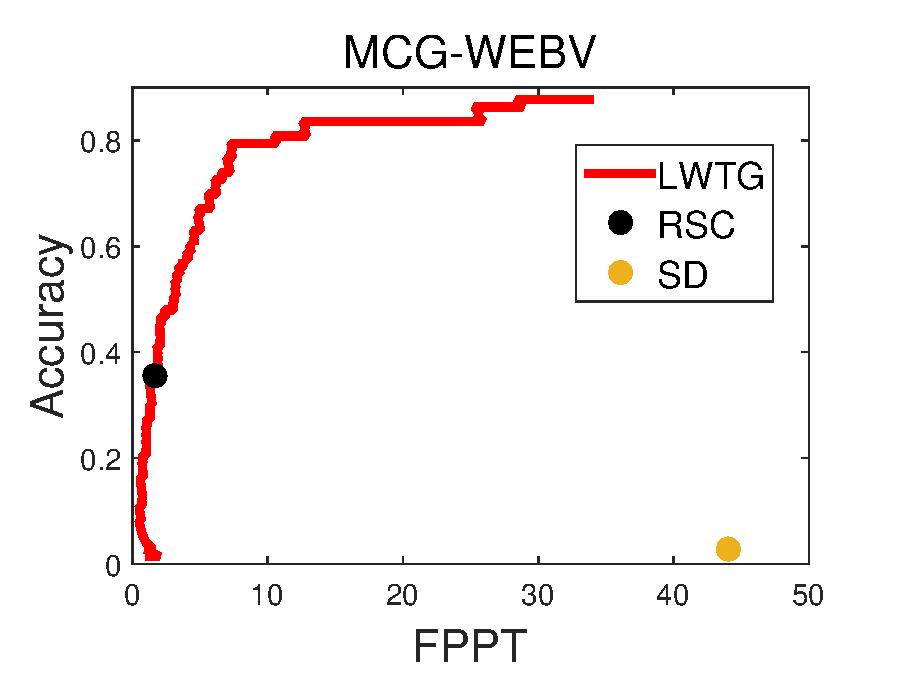
\includegraphics[width=\textwidth,height=0.9\textwidth]{MCG_Accuracy_CMP_denoise}
      \caption{}
      \label{fig:MCG_Accuracy_CMP_denoise}
    \end{subfigure}%
    % ~% add desired spacing
    \begin{subfigure}[b]{0.5\textwidth}
      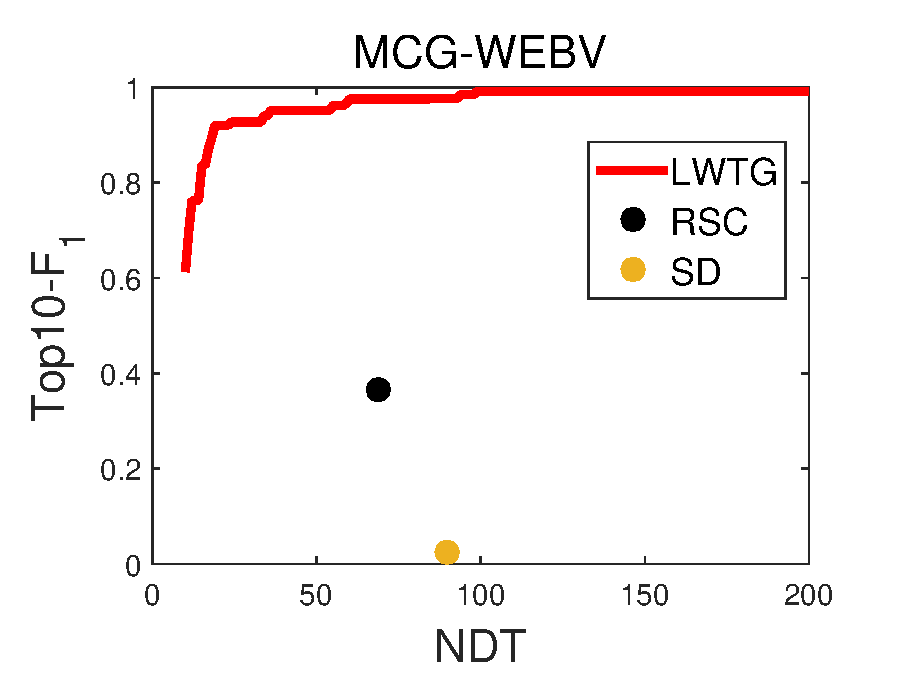
\includegraphics[width=\textwidth,height=0.9\textwidth]{MCG_Top10_CMP_denoise}
      \caption{}
      \label{fig:MCG_Top10_CMP_denoise}
    \end{subfigure}
    \caption{LWTG算法和聚类算法RSC、SD在MCG-WEBV数据集上的对比}
    \label{fig:MCG_CMP_denoise}
\end{figure}
图\ref{fig:MCG_Accuracy_CMP_denoise}和图\ref{fig:MCG_Top10_CMP_denoise}展示了LWTG算法和RSC、SD算法在MCG-WEBV数据集上的实验结果,表明我们的LWTG算法优于SD和RSC算法。从图中可以看出SD算法的$Accuracy$和Top10-$F_1$几乎为0。这是因为在MCG-WEBV数据集中,TF-IDF特征的维度是9,212,这使得SD算法难以有效地从高维和充满噪声的特征中发现聚类。同时,注意到RSC算法在$Accuracy$上跟我们的算法结果相差不大。但是,在Top10-$F_1$上却差很多。这是因为由RSC算法生成的聚类的质量受到大量噪声的影响。而我们的方法不需要复杂的模型构建和优化就能在这两种评测标准上都能取得更好的结果。

\begin{figure}[!htbp]
    \centering
    \begin{subfigure}[b]{0.5\textwidth}
      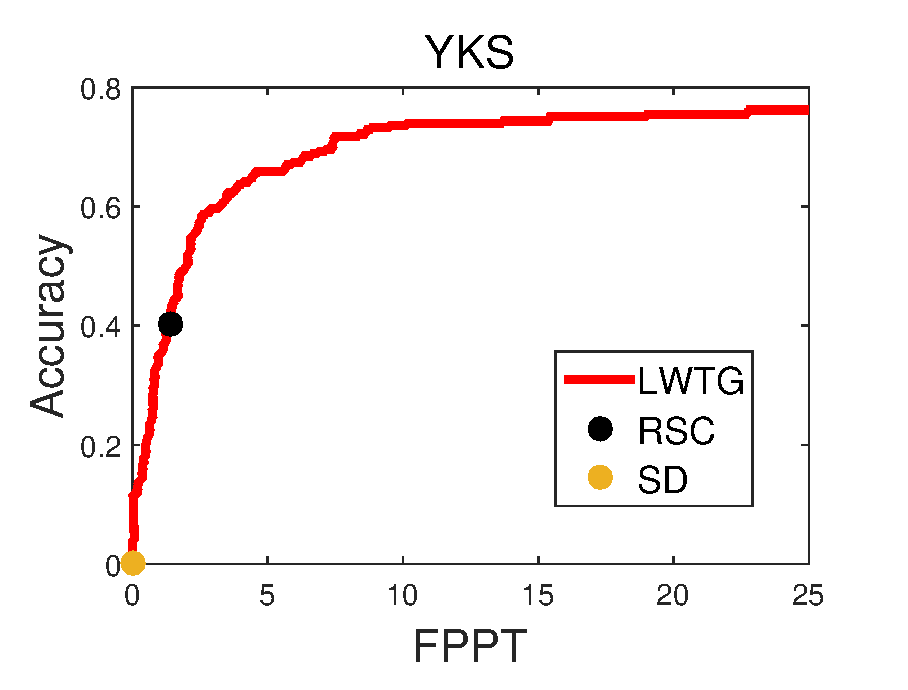
\includegraphics[width=\textwidth,height=0.9\textwidth]{YKS_Accuracy_CMP_denoise}
      \caption{}
      \label{fig:YKS_Accuracy_CMP_denoise}
    \end{subfigure}%
    % ~% add desired spacing
    \begin{subfigure}[b]{0.5\textwidth}
      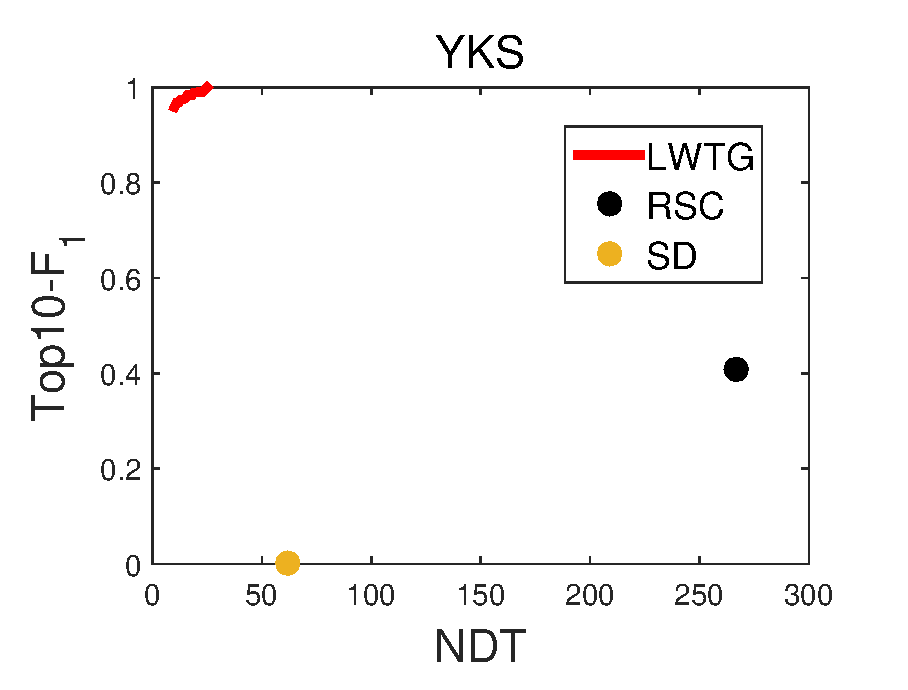
\includegraphics[width=\textwidth,height=0.9\textwidth]{YKS_Top10_CMP_denoise}
      \caption{}
      \label{fig:YKS_Top10_CMP_denoise}
    \end{subfigure}
    \caption{LWTG算法和聚类算法RSC、SD在YKS数据集上的对比}
    \label{fig:YKS_CMP_denoise}
\end{figure}

图\ref{fig:YKS_Accuracy_CMP_denoise}和图\ref{fig:YKS_Top10_CMP_denoise}进一步在YKS数据集上对比LWTG算法和RSC、SD算法。注意到SD算法的实验结果纵轴为0,这是因为YKS数据集的特征维度高达80,294,使得SD方法无法找到任何有效聚类。图\ref{fig:YKS_Accuracy_CMP_denoise}和图\ref{fig:YKS_Top10_CMP_denoise}表明我们的算法在YKS数据集上仍然比RSC和SD算法好。

总之,从话题检测质量来看,在相同话题数量的情况下,我们的LWTG算法在MCG-WEBV和YKS两个数据集上均比RSC和SD方法取得更好的结果。

表\ref{tab:denoisy_time_cmp}进一步在3.6Hz CPU和32G内存的电脑上对比了RSC、SD和LWTG算法的运行时间。虽然在图\ref{fig:MCG_CMP_denoise}和图\ref{fig:YKS_CMP_denoise}中,当FPPT约等于3时,RSC算法的话题准确率和我们的LWTG算法差不多,但是我们的LWTG算法的最终话题召回率远远高于RSC算法。例如表\ref{tab:denoisy_time_cmp}显示我们的LWTG算法在MCG-WEBV数据集上的话题召回率能够高达0.88,而RSC却只能达到0.35。这是因为我们的算法通过多种规模的种子网页来模拟网络话题的L\'evy Walks特性,从而保证了话题检测系统的召回率。

我们同时还注意到当网页从MCG-WEBV数据集的3,600增长到YKS数据集的8,660的时候,RSC算法花了超过15(如:125/8)倍的时间。作为对比,我们的LWTG算法使用了大概5(如:333/73)倍的时间。
\begin{table}[!htbp]
    \caption{不同话题生成算法的运行时间(秒)和系统准确率($Accuracy$)对比}
    \label{tab:denoisy_time_cmp}
    \centering
    \begin{tabular}{|c|c|c|c|}
        \hline
        Data set(\#webpages) & LWTG($Accuracy$) & RSC($Accuracy$) & SD($Accuracy$)\\
        \hline
        \hline
        MCG-WEBV(3660) & $73(\mathbf{0.88})$ & $\mathbf{8}(0.35)$ & $20(0.02)$\\
        \hline
        YKS(8660) & $333(\mathbf{0.77})$ & $\mathbf{125}(0.40)$ & $152(0.00)$\\
        \hline
    \end{tabular}
\end{table}

总之,从话题生成效率来看,虽然我们的LWTG算法比RSC算法慢。但是,当网页数量不断增加时,RSC算法比LWTG算法更加敏感。


\subsection{与网络话题检测算法的对比}

我们对比了LWTG算法与3个优秀的网络话题检测算法:
\begin{enumerate}
  \item[a)] \textbf{Multi-Modality Graph (MMG)\citep{zhang-2013-cross}。} 该算法属于多模态网络话题检测。Zhang等人首先利用视频的NDK信息和文本信息建立相似度图,然后使用图转移算法(Graph Shift,GS)\citep{liu2010graphshift}进行话题检测。MMG假定了一个话题内的元素应该密切相关。所以,通常情况下MMG产生的话题规模较小。
  \item[b)] \textbf{PD with Non-negative Matrix Factorization on Graph
(NMFG)\citep{pang-tao-2018-neurocomputing}。} NMFG和LWTG最大的不同的是产生话题的方式。NMFG中使用基于图的非负矩阵分解(Non-negative Matrix factorization on Graph,NMG\citep{yang2012clustering})在相似度级联上生成过完备话题。NMG算法的聚类非常耗时。
  \item[c)] \textbf{Latent Poisson Deconvolution (LPD) \citep{pang-tao-2016-lpd}。} LPD算法在MCG-WEBV数据集和YKS数据集上均达到了当前最好的性能。相比单纯在PD上使用单一近邻图的方法,LPD利用多个近邻图来排序话题。这个算法证明了我们的算法可以在不利用多个近邻图的情况下达到可接受的结果。
\end{enumerate}

为了尽可能公平的进行对比,在每个数据集上,我们使用了相同的实验设置。
\begin{enumerate}
  \item[1)] \textbf{在MCG-WEBV数据集上进行网络话题生成:} 图\ref{fig:MCG_CMP_webtopics}展示在MCG-WEBV数据集上,我们的LWTG算法和当前几个优秀的网络话题检测算法的对比结果。从图中可以得出以下结论:
  \begin{itemize}
    \item 当FPPT大于8时,LWTG算法显著优于NMFG算法\citep{pang-tao-2018-neurocomputing},几乎能媲美LPD算法\citep{pang-tao-2016-lpd}。但是我们要注意到LPD算法使用非常耗时但是非常有效的NMG算法\citep{yang2012clustering},从两个$k$近邻图中生成话题。而NMFG算法\citep{pang-tao-2018-neurocomputing}也使用NMG算法\citep{yang2012clustering}来生成话题。作为对比,我们提出的LWTG算法避免去设计复杂的模型及其优化。
    \item 当FPPT小与8或者NDT大于200时,LWTG算法稍弱于NMFG算法和LPD算法。主要原因是泊松去卷积算法错误地将不正确的话题排在了正确话题的前面。
  \end{itemize}

  \begin{figure}[!htbp]
    \centering
    \begin{subfigure}[b]{0.5\textwidth}
      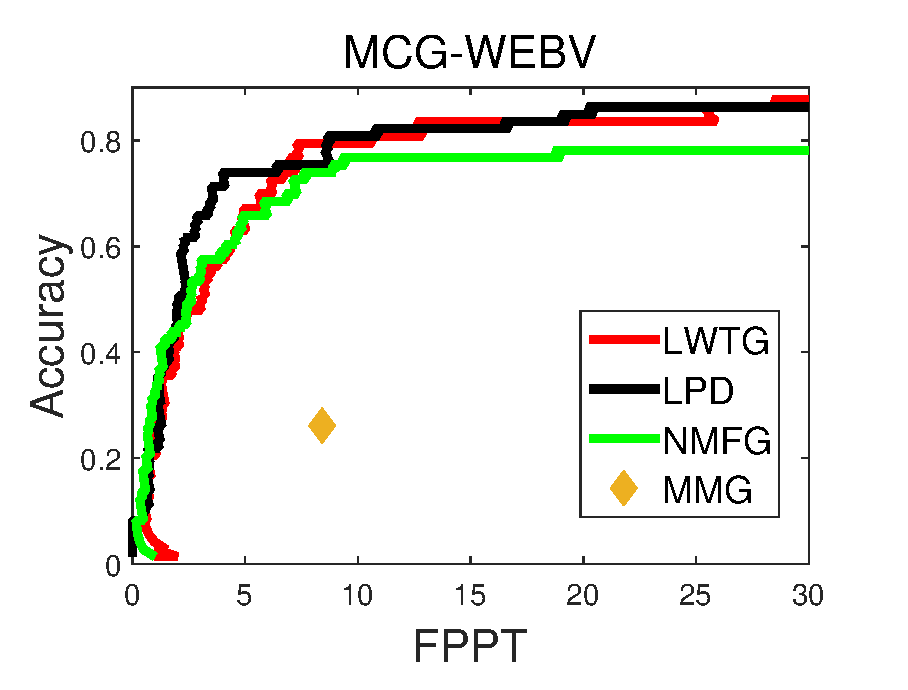
\includegraphics[width=\textwidth,height=0.9\textwidth]{MCG_Accuracy_CMP_webtopics}
      \caption{}
      \label{fig:MCG_Accuracy_CMP_webtopics}
    \end{subfigure}%
    % ~% add desired spacing
    \begin{subfigure}[b]{0.5\textwidth}
      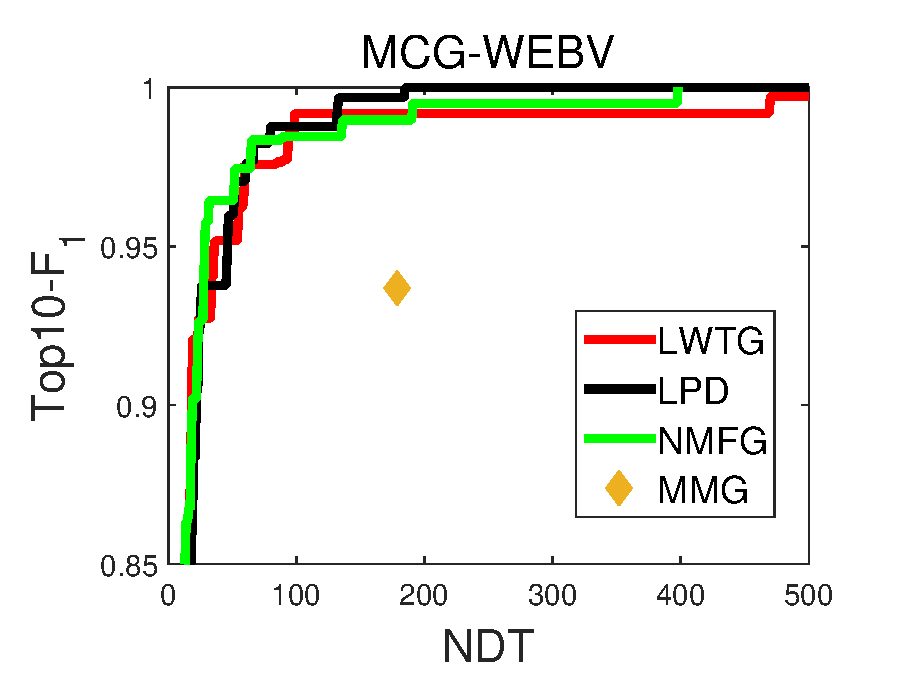
\includegraphics[width=\textwidth,height=0.9\textwidth]{MCG_Top10_CMP_webtopics}
      \caption{}
      \label{fig:MCG_Top10_CMP_webtopics}
    \end{subfigure}
    \caption{LWTG算法和其他网络话题检测算法在MCG-WEBV数据集上的对比}
    \label{fig:MCG_CMP_webtopics}
  \end{figure}
  就话题生成效率来看,表\ref{tab:webtopics_time_cmp}显示NMFG和LPD算法的运行时间分别是LWTG算法的71(如:5248/73)和158(如:11545/73)倍。这意味着我们的LWTG算法非常有希望能很好地对大规模网络数据进行快速的网络话题生成。与此同时,LWTG算法的话题检测的有效性也比得上当前最优秀的算法。
  \begin{table}[!htbp]
      \caption{不同话题生成算法的运行时间(秒)和生成的话题数量对比}
      \label{tab:webtopics_time_cmp}
      \centering
      \begin{tabular}{|c|c|c|c|c|}
      % \begin{tabular}{|p{4cm}<{\centering}|p{1cm}<{\centering}|p{1cm}<{\centering}|p{2.5cm}<{\centering}|p{1cm}<{\centering}|p{3cm}<{\centering}|}
          \hline
          Data set(\#topic) & LWTG(\#topic) & LPD(\#topic) & NMFG(\#topic) & MMG(\#topic)\\
          \hline
          \hline
          MCG-WEBV(3660) & $\mathbf{73}(\mathbf{2504})$ & $11545(7685)$ & $5248(4238)$ & $15(430)$\\
          \hline
          YKS(8660) & $\mathbf{333}(7458)$ & $29321(7524)$ & $13847(\mathbf{5714})$ & 2$52(445)$\\
          \hline
      \end{tabular}
  \end{table}

  \item[2)] \textbf{在YKS数据集上进行网络话题生成:} YKS是一个跨平台的数据集,比MCG-WEBV数据集包含更多不同类型的话题,也更有挑战性。图\ref{fig:YKS_CMP_webtopics}进一步说明了当FPPT大于8时,我们提出的LWTG算法仍然显著优于当前最好的话题检测算法。

  \begin{figure}[!htbp]
    \centering
    \begin{subfigure}[b]{0.5\textwidth}
      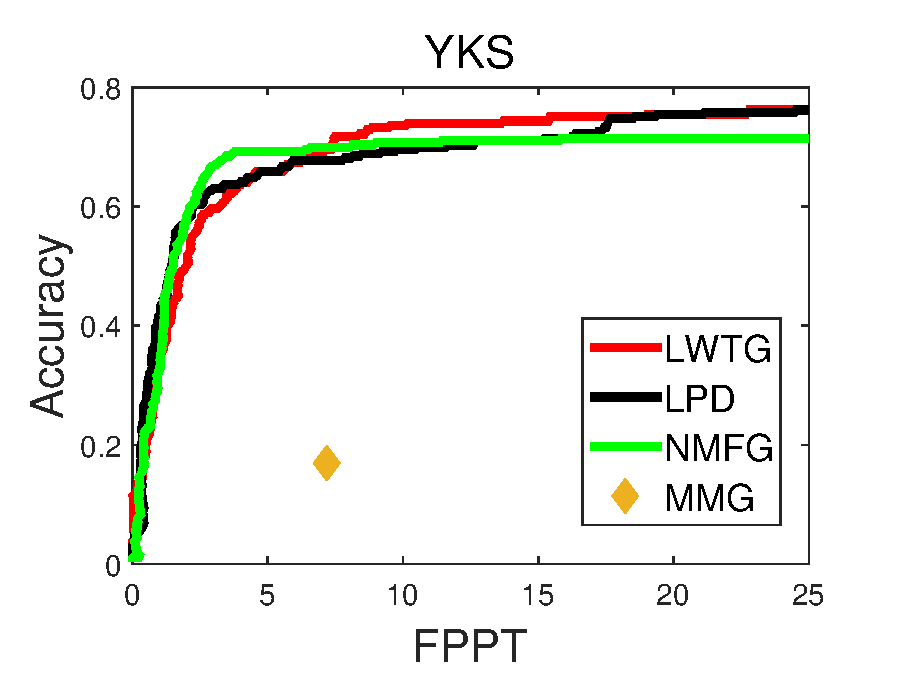
\includegraphics[width=\textwidth,height=0.9\textwidth]{YKS_Accuracy_CMP_webtopics}
      \caption{}
      \label{fig:YKS_Accuracy_CMP_webtopics}
    \end{subfigure}%
    % ~% add desired spacing
    \begin{subfigure}[b]{0.5\textwidth}
      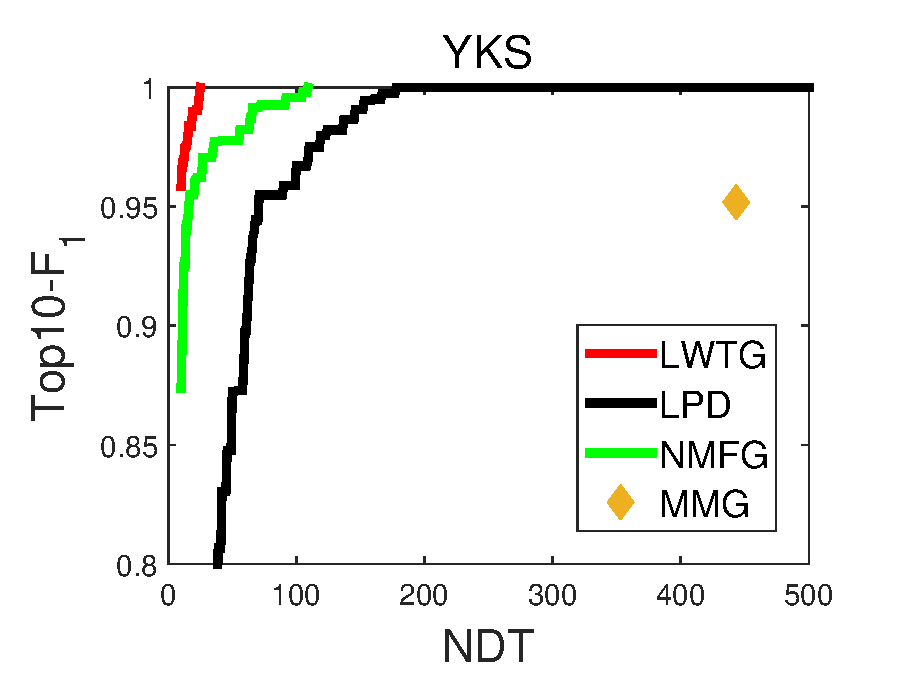
\includegraphics[width=\textwidth,height=0.9\textwidth]{YKS_Top10_CMP_webtopics}
      \caption{}
      \label{fig:YKS_Top10_CMP_webtopics}
    \end{subfigure}
    \caption{LWTG算法和其他网络话题检测算法在YKS数据集上的对比}
    \label{fig:YKS_CMP_webtopics}
  \end{figure}
  同时就话题生成效率来看,表\ref{tab:webtopics_time_cmp}显示了NMFG和LPD算法的运行时间分别是LWTG算法的41(如:13847/333)和88(如:29321/333)倍。这同样意味着我们的LWTG算法非常有希望能很好地对大规模网络数据进行快速的网络话题生成。虽然MMG算法的运行时间比较低,但是该算法对网页数量非常敏感。比如说当网页数量从MCG-WEBV数据集的3,660增长到YKS数据集的8,660的时候,数据集只增长2.4(如:8660/3660)倍,但是,MMG算法的运行时间超过了16(如:252/15)倍。同时,MMG算法对于网络话题检测的效果也远远不如其他几个算法。
\end{enumerate}


\section{小结}

本章介绍了一种面向网络数据的快速生成网络话题的算法,有望解决基于大规模网络数据的话题检测问题。该算法通过对网页计算其属于话题中心网页的概率来排序网页,进而生成不同规模的种子网页。然后模拟网络话题的L\'evy Walks特性,定义网页-种子话题之间的相似度,采用一种基于种子话题的网页多分配算法来生成话题,同时使用层级阈值来截断话题,最终生成一系列过完备的话题。最后的实验从话题生成效果和话题生成效率两方面验证了我们提出的LWTG算法的优越性。

